\documentclass[final]{siamltex}
%test change
\usepackage{cite}
\usepackage{graphicx,bbm,pstricks,soul}
\usepackage{pifont}
\usepackage{bbm,algorithmic,mdframed,placeins,multirow,booktabs,subfigure}
\usepackage[ruled,vlined,linesnumbered]{algorithm2e}
\usepackage{tikz,hhline}
\usetikzlibrary{positioning,automata}
\usetikzlibrary{arrows,fit}
\usetikzlibrary{decorations.pathmorphing}
\usepackage{tabularx}
\newcolumntype{L}[1]{>{\raggedright\let\newline\\\arraybackslash\hspace{0pt}}m{#1}}
\newcolumntype{C}[1]{>{\centering\let\newline\\\arraybackslash\hspace{0pt}}m{#1}}
\newcolumntype{R}[1]{>{\raggedleft\let\newline\\\arraybackslash\hspace{0pt}}m{#1}}

\let\oldnl\nl% Store \nl in \oldnl
\newcommand{\nonl}{\renewcommand{\nl}{\let\nl\oldnl}}% Remove line number for one line

\setlength{\parindent}{0in}
\usepackage{amsmath,amsfonts,amsbsy,amssymb}
\newcommand{\RARR}[3]{#1
  \;\displaystyle\mathop{\displaystyle\longrightarrow}^{#3}\; #2}
\newcommand{\RARRlong}[3]{#1
  \;\displaystyle\mathop{-\!\!\!-\!\!\!-\!\!\!-\!\!\!-\!\!\!\!\displaystyle
  \longrightarrow}^{#3}\; #2}
\newcommand{\LARR}[3]{#1
  \;\displaystyle\mathop{\displaystyle\longleftarrow}^{#3}\; #2}
\newcommand{\LRARR}[4]{{\mbox{ \raise 0.4 mm \hbox{$#1$}}} \;
  \mathop{\stackrel{\displaystyle\longrightarrow}\longleftarrow}^{#3}_{#4}
  \; {\mbox{\raise 0.4 mm\hbox{$#2$}}}}
\newcommand{\bX}{{\bf X}}
\newcommand{\vecx}{{\mathbf x}}
\newcommand{\vecy}{{\mathbf y}}
\newcommand{\vecz}{{\mathbf z}}
\newcommand{\vecq}{{\mathbf q}}
\newcommand{\bs}{{\mathbf s}}
\newcommand{\vecr}{{\mathbf r}}
\newcommand{\vecX}{{\mathbf X}}
\newcommand{\vecv}{{\mathbf v}}
\newcommand{\tick}{\ding{52}}
\newcommand{\cross}{\ding{54}}
\newcommand{\vecn}{{\mathbf n}}
\newcommand{\vecp}{{\mathbf p}}
\newcommand{\cT}{{\mathcal T}}
\newcommand{\dt}{{\mbox{d}t}}
\newcommand{\dx}{{\mbox{d} \vecx}}
\newcommand{\boldnu}{{\boldsymbol \nu}}
\newcommand{\er}{{\mathbb R}}
\renewcommand{\div}{{\rm div}}
\newcommand{\bnu}{{\bf \nu}}
\newcommand{\divergence}{\mathop{\mbox{div}}}
\renewcommand{\P}{\mathbb{P}}
\newcommand{\FP}{P_{\rm{FP}}}
\newcommand{\ME}{P_{\rm{ME}}}
\newcommand{\MEs}{P_{\rm{ME}_{S}}}
\newcommand{\D}{\mathcal{D}}
\newcommand{\G}{\mathcal{G}}
\newcommand{\N}{\mathcal{N}}
\newcommand{\X}{{\mathbf X}}
\newcommand{\Y}{{\mathbf Y}}
\newcommand{\W}{{\mathbf W}}
\newcommand{\data}{D}
\newcommand{\neff}{n_{\text{eff}}}
\newcommand{\E}{{\mathbb E}}
\renewcommand{\b}[1]{{\bf #1}}
\DeclareMathOperator*{\argmin}{arg\,min}
\DeclareMathOperator*{\argmax}{arg\,max}

\newcommand{\picturesAB}[6]{
\centerline{
\hskip #4
\raise #3 \hbox{\raise 0.9mm \hbox{(a)}}
\hskip #5
\epsfig{file=#1,height=#3}
\hskip #6
\raise #3 \hbox{\raise 0.9mm \hbox{(b)}}
\hskip #5
\epsfig{file=#2,height=#3}
}}
\newcommand{\picturesCD}[6]{
\centerline{
\hskip #4
\raise #3 \hbox{\raise 0.9mm \hbox{(c)}}
\hskip #5
\epsfig{file=#1,height=#3}
\hskip #6
\raise #3 \hbox{\raise 0.9mm \hbox{(d)}}
\hskip #5
\epsfig{file=#2,height=#3}
}}

\makeatletter  
\newcommand{\xleftrightarrows}[2][]{\mathrel{%  
 \raise.40ex\hbox{$  
       \ext@arrow 3095\leftarrowfill@{\phantom{#1}}{#2}$}%  
 \setbox0=\hbox{$\ext@arrow 0359\rightarrowfill@{#1}{\phantom{#2}}$}%  
 \kern-\wd0 \lower.4ex\box0}}  
 
\newcommand{\xrightleftarrows}[2][]{\mathrel{%  
 \raise.40ex\hbox{$\ext@arrow 3095\rightarrowfill@{\phantom{#1}}{#2}$}%  
 \setbox0=\hbox{$\ext@arrow 0359\leftarrowfill@{#1}{\phantom{#2}}$}%  
 \kern-\wd0 \lower.4ex\box0}}  
 
\def\leftrightarrowfill@{%
 \arrowfill@\leftarrow\relbar\rightarrow%
 }
\newcommand*{\centerfloat}{%
  \parindent \z@
  \leftskip \z@ \@plus 1fil \@minus \textwidth
  \rightskip\leftskip
  \parfillskip \z@skip}
\makeatother
\makeatother 

\newcommand\irregularcircle[2]{% radius, irregularity
  \pgfextra {\pgfmathsetmacro\len{(#1)+rand*(#2)}}
  +(0:\len pt)
  \foreach \a in {10,20,...,350}{
    \pgfextra {\pgfmathsetmacro\len{(#1)+rand*(#2)}}
    -- +(\a:\len pt)
  } -- cycle
}

\newcommand{\into}{\operatornamewithlimits{\longrightarrow}}
\newtheorem{dfn}{Definition}[section]

\newcommand{\ltri}{%
\,\resizebox{!}{0.25\baselineskip}{%
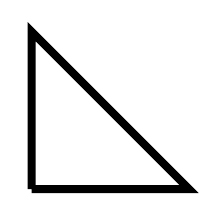
\begin{tikzpicture}%
\draw[line width=1mm](0,0) -- (0,2) -- (2,0)  -- (0,0);
\end{tikzpicture}%  
}\xspace%
}%

\newcommand{\smallltri}{%
\,\resizebox{!}{0.15\baselineskip}{%
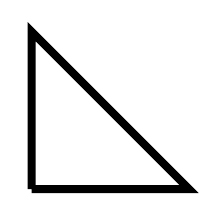
\begin{tikzpicture}%
\draw[line width=1mm](0,0) -- (0,2) -- (2,0)  -- (0,0);
\end{tikzpicture}%  
}\xspace%
}%

\title{Transport map accelerated-PAIS, and application to inverse problems arising from
  multiscale stochastic reaction networks}
\author{Simon Cotter, Yannis Kevrekidis, Paul Russell}
\begin{document}
\maketitle
\begin{abstract}
In many applications, inverse problems arise where where there are
complex correlations between the different parameters which we wish to
infer from data. The correlations often manifest themselves as lower
dimensional manifolds on which the likelihood function is
invariant, or varies very little. This can be due to trying to infer
unobservable parameters, or due to sloppiness in the model which is
being used to describe the data. In such a situation, standard
sampling methods for characterising the posterior distribution which
do not incorporate information about this structure will be highly
inefficient. Moreover, most methods are inherently serial in nature,
and as such are not expoiting the parallelised  nature of modern
computer infrastructure. In this paper, we seek to develop a method to
tackle this problem, using optimal transport maps to simplify
posterior distributions which are concentrated on lower dimensional
manifolds.

We demonstrate the approach by considering inverse problems arising
from partially observed stochastic reaction networks. In particular,
we consider systems which exhibit multiscale behaviour, but for which
only the slow variables in the system are observable. We demonstrate
that certain multiscale approximations lead to more consistent
approximations of the posterior than others.
\end{abstract}


\section{Introduction}
%Topics to cover: parallel MCMC, pMC, PAIS
%Transport maps, transport map MCMC
%Stochastic reaction networks
%Multiscale approximations, QSSA/QEA, CMA

In Section \ref{sec:map} we show how an appropriate transport map can
be constructed from importance samples which maps the posterior close
to a reference Gaussian measure. In Section \ref{sec:TPAIS} we show
how such a map can be incorporated into a sophisticated parallel MCMC
infrastructure in order to accelerate mixing. In Section
\ref{sec:multi} we consider how likelihoods can be approximated using
multiscale methodologies in order to carry out inference for
multiscale and/or partially observed stochastic reaction networks. In
Section \ref{sec:num} we present some numerical examples, which serve
to demonstrate the increased efficiency of the described sampling
methodologies, as well as investigating the posterior approximations
discussed in the previous section. We conclude with a discussion in
Section \ref{sec:conc}.


\section{Construction of transport maps in importance sampling} \label{sec:map}
%Follow the other papers, show adaptation(s)

So far we have seen that the PAIS algorithm is efficient for low dimensional posterior sampling.
PAIS is particularly useful if the posterior is multimodal, or inconveniently shaped such as the
Rosenbrock density discussed in Chapter~\ref{sec:LPAIS}. However, we have had trouble when
attempting to increase the dimension of the parameter space. This was seen when we attempted to
recover the initial condition for the wave equation in Chapter~\ref{sec:PAIS}.

In this Chapter we look at a method which will allow us to improve efficiency in our proposal distributions. The ideal sampling
situation in MCMC is to explore an $d$-dimensional Gaussian distribution (or other standard distribution) using a near proportional
proposal distribution. We therefore aim to transform an arbitrary distribution, $\mu_\theta$, in to a Gaussian distribution, which we can then sample from efficiently, and finally transform this sample back into a sample from $\mu_\theta$. In this way we hope to be able to sample from any distribution $\mu_\theta$ with a similar efficiency as we obtain when sampling from a Gaussian distribution. In particular for the PAIS algorithm, resampling schemes are more efficient in higher
dimensions if the dimensions are uncorrelated. The work of Moselhy and
Marzouk~\cite{el2012bayesian}, Parno and Marzouk~\cite{parno2014transport} and
Parno~\cite{parno2015transport} provides a method of constructing such a map as part of an adaptive
Metropolis-Hastings algorithm.

%Given some constraints it is computationally tractable to adaptively construct invertible maps
%during an MCMC simulation. These maps construct a continuous coupling between a target and
%reference distribution, where the latter is chosen to be a standardised Gaussian. How close this reference
%distribution is to Gaussian depends on three considerations; firstly the constraints applied. These
%constraints, discussed later, ensure that the map exists, is unique, and is invertible. The
%necessity for the map to be invertible, and preferrably easily invertible, restricts the space of
%possible couplings to the point where it is unlikely that the exact map is included in our space of
%feasible transference plans. Secondly, for our purposes, the map takes the form of a polynomial
%chaos expansion which requires infinitely many terms to exactly represent the coupling. This is of course not possible on current hardware. Finally we
%will be constructing this map using an optimisation problem where the objective function depends on
%the sample path of our MCMC algorithm. This sample does not represent the target exactly until $N\rightarrow\infty$, and so the expectation is only calculated approximately.
%
%While the restrictions on the map are essential for well-posedness, the approximate map which
%results from these constraints can be made arbitrarily accurate by increasing the number of basis
%functions used in the expansion, and increasing the number of samples used in the optimisation
%problem. In practice it appears that we need not aim to achieve a high accuracy solution. Excellent
%results have been observed using monomial basis functions of total order 3, and we need a sample of
%size of only $\mathcal{O}(10^3)$ to obtain a well converged map.

In~\cite{el2012bayesian} the transport map was introduced to provide a transformation from the prior
distribution to the posterior distribution, the idea being that one could draw a moderately sized
sample from the prior distribution and use this sample to approximate a map onto the target space.
Once this map was known to the desired accuracy a larger sample from the prior could be used to
investigate the posterior distribution. This
methodology was adapted in~\cite{parno2014transport} to form a new proposal method for MH
algorithms. In this case, rather than transforming a sample from the prior into a sample from the target
distribution, the map transforms a sample from the posterior onto a reference space.
The reference density is chosen to allow efficient proposals using a simple proposal
distribution such as a Gaussian centred at the previous state. Proposed states can then be mapped back into a sample from the posterior by applying the inverse of the transport map.

Proposing new states in this way allows us to make large steps around complex probability distributions.
It is also feasible in this framework to assume that the reference density is close enough to a standard Gaussian that we can efficiently propose moves using a proposal distribution which is independent of the current state, e.g. choose $q(\theta) = \mathcal{N}(0,I_n)$.

In this chapter we introduce the derivation of the map discussed, show how it can be adapted to work
with a weighted sample, and that mixture distributions as used in the PAIS algorithm can more
efficiently approximate the reference space and so lead to higher overall effective sample sizes.
Further we show that the algorithm arising from the combination of these methods can lead to more
efficient sampling than either can achieve on its own.

\section{The Transport Map}

In this section we outline the methodology in \cite{parno2014transport} for coupling the target,
$\mu_{\theta}$, with the reference distribution, $\mu_r$.
We also show how the map can be constructed using a weighted sample and hence how we can incorporate the map into the PAIS algorithm.

\begin{dfn}[Transport Map $T$]
	Given a probability distribution $\mu_\theta$ with support $\mathcal{X}$.
	A transport map is a function $T\colon \mathcal{X} \rightarrow \mathbb{R}^d$ such that
	\[
		\mu_\theta(A) = \mu_r(T(A)) \quad \text{for any } A \subset \mathcal{X}.
	\]
\end{dfn}

\begin{dfn}[Exact Transport Map $T$]
	A transport map $T$ is exact if the {\it pullback} of the standard Gaussian density, $\phi(\cdot)$,
	\begin{equation}\label{eq:pullback}
		\tilde{\pi}(\theta) = \phi(T(\theta))|J_T(\theta)|,
	\end{equation}
	is equal to the target density $\pi(\theta)$ for all $\theta \in \mathcal{X}$. The pullback is defined in terms of the determinant of the Jacobian of $T$,
	\[
		|J_T(\theta)| = \text{det}\begin{bmatrix} \partial_{\theta_1} T_1(\theta) & \dots & \partial_{\theta_d} T_1(\theta) \\ \vdots & \ddots & \vdots \\ \partial_{\theta_1} T_d(\theta) & \dots & \partial_{\theta_d} T_d(\theta) \end{bmatrix}.
	\]
\end{dfn}

In the case that we have the exact map, $T\in\mathcal{T}$ where $\mathcal{T}$ is the space of all invertible maps, we are able to draw a sample from $\pi_r = \phi$, the density of the standardised Gaussian distribution, and map these samples back onto target space using $T^{-1}$. These proposed samples are distributed according to the target distribution.

\begin{dfn}[Target and Reference Space]
	The transport map pushes a particle from a {\it target space} $\mathcal{X}$, that is a subset of $\mathbb{R}^d$ equipped with a target measure $\mu_{\theta}$, onto a {\it reference space}, $R$, again a subset of $\mathbb{R}^d$ equipped with the reference measure $\mu_r$.
\end{dfn}

On target space, the proposal density is induced by the pullback of $\phi$ through $T^{-1}$.
Clearly the pullback only exists when $T$ is monotonic and has continuous first derivatives.
Not all maps satisfy these conditions, so we define a smaller space of maps, $\mathcal{T}^\uparrow \subset \mathcal{T}$ which contains all feasible maps.
The exact map $T$ is not necessarily in $\mathcal{T}^\uparrow$, so we are motivated to formulate an optimisation problem as discussed in Section~\ref{sec:intro_optim}.

We attempt to find a deterministic coupling of two continuous probability distributions, $(\mu_\theta, \mu_r)$, such that $\mu_r = T\mu_\theta$ is satisfied and also that $T \in \mathcal{T}^\uparrow$. There may be infinitely many such couplings, so we look to find the coupling which minimises the KL-divergence between the density of $\mu_{\theta}$ and the pullback of the density of $\mu_{r}$, i.e. the distance between $\pi(\theta)$ and $\tilde{\pi}(\theta)$.

When we optimise the cost function
\[
	C(T) = D_\text{KL}(\pi\|\tilde{\pi}),
\]
numerically, it is not guaranteed that the resulting map will be invertible, so it must be enforced in the design of each map component. To ensure invertibility we restrict the map to be lower triangular, i.e. $\tilde{T} \in \mathcal{T}^{\ltri}\subset\mathcal{T}^\uparrow$. This lower triangular map has the form,
\[
	T(\theta_1, \dots, \theta_n) = \begin{bmatrix} T_1(\theta_1) \\ T_2(\theta_1, \theta_2) \\ \vdots \\
		T_n(\theta_1, \dots, \theta_n) \end{bmatrix},
\]
where $T_i\colon \mathbb{R}^i \to \mathbb{R}$. We assume that the target and reference probability densities are absolutely continuous on
$\mathbb{R}^d$. Under this formulation we are guaranteed a unique invertible map $\tilde{T}$ with the property that
\[
	\tilde{T}\mu_{\theta} \approx \mu_r.
\]
Relaxing the equality constraint to finding the approximate map $\tilde{T} \in \mathcal{T}^{\ltri}$ which optimises $C(T)$, allows us to formulate an efficient sampling method, in terms of the linear algebra required, and experimentation has shown that the pushforward of the target is close enough to Gaussian to achieve efficient sampling.

\subsection{The optimisation problem}

With these constraints in mind we formulate the optimisation problem explicitly. The cost function
is chosen to be the Kullback-Leibler divergence between the posterior density and the pullback density,
\[
	D_\text{KL}(\pi\|\tilde{\pi}) =
		\mathbb{E}_\pi\left[\log\left(\frac{\pi(\theta)}{\tilde{\pi}(\theta)}\right)\right].
\]
This divergence results in some nice properties which we will explore in the following derivation. The KL divergence is not a true metric since it is not symmetric, however it is commonly used to measure the distance between probability distributions due to it's relatively simple form, and because it provides a bound for the square of the Hellinger distance by Pinsker's inequality~\cite{pinsker1960information},
\[
	D_{KL}(p\|q) \geq D_H^2(p,q),
\]
which is a true metric between probability distributions $p$ and $q$.
Given the form of the pullback in Equation~\eqref{eq:pullback}, now taken through an approximate map $\tilde{T}$, the divergence becomes
\[
	D_\text{KL}(\pi\|\tilde{\pi}) = \mathbb{E}_\pi\left[\log\pi(\theta) - \log\pi_r(\tilde{T}(\theta)) -
		\log\left|J_{\tilde{T}}(\theta)\right|\right].
\]
We note the posterior density is independent of $\tilde{T}$, and so it is not necessary for us to compute it when optimising this cost function. This expression is a complicated integral with respect to the target distribution, for which the normalisation constant is unknown. However this is exactly the scenario for which we would turn to MCMC methods for a solution.

To find the best coupling, $\tilde{T} \in \mathcal{T}^{\ltri}$, we solve the optimisation problem,
\[
	\tilde{T} = \arg\min_{T \in \mathcal{T}^{\smallltri}} \mathbb{E}_\pi\left[-\log\pi_r(T(\theta)) -
		\log\left|J_T(\theta)\right|\right]
\]
which has a unique solution since the cost function is convex.

We also include a regularisation term which is required for reasons which will become clear later. The optimisation problem now takes the form
\begin{equation}\label{eq:gen_map_optim}
	\tilde{T} = \arg\min_{T\in\mathcal{T}^{\smallltri}} \left[
		 \mathbb{E}_\pi\left[-\log\pi_r(T(\theta)) -
		\log\left|J_T(\theta)\right|\right] + \beta\mathbb{E}(T(\theta)- \theta)^2 \right].
\end{equation}
This parameter $\beta$ does not need to be tuned, experimentation has shown that the choice
$\beta=1$ is sufficient for most problems. The form of the penalisation term promotes maps which are
closer to the identity.

\subsection{The structure of the map}

Before we continue with the derivation of the optimisation problem, we consider the structure
of the map in more detail. The lower triangular structure of the map not only guarantees monotonicity, it also allows for efficient calculation of the pullback density, as well as the inverse of the map, $\tilde{T}^{-1}$. The Jacobian of $\tilde{T}$ is a lower triangular matrix,
\[
	J_T(\theta) = \begin{bmatrix}
		\partial_{\theta_1} \tilde{T}_1(\theta) & \dots & \partial_{\theta_d} \tilde{T}_1(\theta)\\
		\vdots & \ddots & \vdots \\
		\partial_{\theta_1} \tilde{T}_d(\theta) & \dots & \partial_{\theta_d} \tilde{T}_d(\theta)
	\end{bmatrix} = \begin{bmatrix}
		\partial_{\theta_1} \tilde{T}_1(\theta) & \dots & 0\\
		\vdots & \ddots & \vdots \\
		\partial_{\theta_1} \tilde{T}_d(\theta) & \dots & \partial_{\theta_d} \tilde{T}_d(\theta)
	\end{bmatrix}
\]
since $\partial_{\theta_n} \tilde{T}_k(\theta) = 0$ for all $n > k$. This lower triangular structure means that the determinant of the Jacobian is a product of the diagonal elements which, when we take logs, becomes
\begin{equation}\label{eqn:separable_jacobian}
	\log\left|J_{\tilde{T}}(\theta)\right| = \sum\limits_{i=1}^d \! \log \partial_{\theta_i} \tilde{T}_i(\theta).
\end{equation}
Here we note that this term is separable in terms of the dimension $i$.

%Inverting $T$ is simplified by the lower triangular structure in the sense that in each dimension, $i$, we need only invert a univariate polynomial. This simplification comes about because we invert each dimension of the map independently, beginning with $T_1$ which is a function of only $\theta_1$. Finding the root of $T_1(\theta_1) = r_1$, gives us the value of $\theta_1$ which we can then use to find the root of $T_2(\theta_2;\theta_1) = r_2$, and so on. These roots, $r_1,\dots,r_d$, are restricted to be real since $\mathcal{X} \subset \mathbb{R}^d$, which allows us to find the unique point, $\theta$, which corresponds to the point $r$.

Inverting $\tilde{T}$ at a point $r$ is simplified by the lower triangular structure of the map. The map component $\tilde{T}_1(\theta)$ is a univariate polynomial in $\theta_1$, so we can find the inverse of this function by solving the equation $T_1(\theta_1) = r_1$. This inversion tells us the value of $\theta_1$, which means the next component is again a univariate polynomial, $T_2(\theta_2; \theta_1)=r_2$. We can then perform $d$ root finding problems instead of a full $d$ dimensional non-linear solve.

We require that the first derivatives of the map are continuous, which is easy to enforce by the choice of basis functions. Here we assume that the map will be built from a family of orthogonal polynomials, $\mathcal{P}(\theta)$, not necessarily orthogonal with respect to the target distribution. Each component of the map is defined as a multivariate polynomial expansion,
\begin{equation}\label{eq:map_defn}
	\tilde{T}_i(\theta; \gamma_i) = \sum\limits_{\mathbf{j}\in\mathcal{J}_i} \!
\gamma_{i,\mathbf{j}}\psi_\mathbf{j}(\theta).
\end{equation}
The parameter $\gamma_i$ is a vector of coefficients in $\mathbb{R}^{M_i}$. Each component of $\gamma_i$ corresponds to a basis function
$\psi_\mathbf{j}$, indexed by the multi-index $\mathbf{j} \in \mathbb{N}_0^d$. These multi-indices are elements of the multi-index set $\mathcal{J}_i$. A multi-index defines a product of univariate polynomials in $\theta_k$,
\[
	\psi_\mathbf{j}(\theta) = \prod\limits_{k=1}^i \! \varphi_{j_k}(\theta_k), \quad \text{for} \quad \mathbf{j} \in \mathcal{J}_i,
\]
and where $\varphi_{j_k}(\theta_k) \in \mathcal{P}(\theta_k)$. Since $\tilde{T}$ is lower triangular, a multi-index $\mathbf{j}\in\mathcal{J}_i$ only contains entries for univariate polynomials in $\theta_k$ for $k\leq i$.

The cardinalities of the multi-index sets, $M_i = \text{card}(\mathcal{J}_i)$, give the number of unknowns in our
optimisation problem, and so we would like to keep this number as small as possible. One option is
to use polynomials of total order $p$,
\[
	\mathcal{J}_i^\text{TO} = \left\{\mathbf{j}:\|\mathbf{j}\|_1 \leq p, j_k = 0\ \forall k > i\right\},
\]
which is optimal in terms of the amount of information captured by the map about the target. The cardinality of $\mathcal{J}_i^\text{TO}$ is $M_i = {i+p \choose p}$ which increases rapidly in $d$ and $p$, where $i = 1, \dots, d$. Smaller optimisation problems can be produced by constructing subsets of $\mathcal{J}_i^\text{TO}$. These index sets are discussed
in~\cite{parno2014transport}. Increased information with a slower increase in the number of map parameters can be achieved with the composition of maps discussed in~\cite{parno2015transport}. Here we stick with polynomials of total order $p$ since we work with low dimensional problems with the PAIS algorithm.


\subsection{Implementation of the optimisation problem}\label{sec:transport_implementation}

We now discuss how we can evaluate Equation~\eqref{eq:gen_map_optim} using a sample from the target distribution. We first reformulate the expectation in the cost functional in terms of a MC estimator,
\begin{align}
	C(T) &= \mathbb{E}_\pi\left[ -\log\pi_r(T(\theta)) - \log|J_T(\theta)|\right] +
			\beta\mathbb{E}(T(\theta)-\theta)^2 \notag \\
		&\approx \frac{1}{K}\sum\limits_{i=1}^d \! \sum\limits_{k=1}^K \left[-\log\pi_r(T_i(\theta^{(k)})) -
			\log\left|\frac{\partial T_i}{\partial \theta_i}(\theta^{(k)})\right| + \beta(T_i(\theta^{(k)})-\theta^{(k)})^2\right]. \label{eqn:TM_full_cost}
\end{align}
Optimisation of this cost function results in a map from $\pi$ to some reference density $\pi_r$. By choosing the reference density to be a Gaussian density, we can simplify this expression greatly. Substitution of the Gaussian density into Equation~\eqref{eqn:TM_full_cost} leads to
\begin{equation}\label{eq:gauss_map_optim}
	C(T) = \frac{1}{K}\sum\limits_{i=1}^d \! \sum\limits_{k=1}^K \left[\frac{1}{2}
		T_i^2(\theta^{(k)}) - \log\frac{\partial T_i}{\partial \theta_i}(\theta^{(k)}) +
		\beta(T_i(\theta^{(k)})-\theta^{(k)})^2\right].
\end{equation}
Note that since we assume that the map is monotonic, the derivatives of each component are
positive and so this functional is always finite. In practice it is infeasible to enforce this condition across the whole parameter space. We instead enforce this condition by ensuring that the derivatives are positive at each sample point. This means that when we sample away from these support points while in reference space, it is possible to enter a region of space where the map is not monotonic.

We now return to the structure of the map components given in Equation~\eqref{eq:map_defn}. Since the basis functions are
fixed, the optimisation problem in \eqref{eq:gen_map_optim} is really over the map components $\bar{\gamma} = (\gamma_1, \dots,
\gamma_d)$ where $\gamma_i \in \mathbb{R}^{M_i}$. Note that $C(T)$ is the sum of $d$ expectations, and these expectations each only concern one dimension. Therefore we can rewrite \eqref{eq:gen_map_optim} as $d$ separable optimisation problems.
\begin{align}\label{eq:gamma_map_optim}
	&\arg\min_{\gamma_i\in\mathbb{R}^{M_i}} \frac{1}{K}\sum\limits_{k=1}^K
		\left[\frac{1}{2}T_i^2(\theta^{(k)}; \gamma_i) - \log\frac{\partial T_i}{\partial\theta_i}(\theta^{(k)}; \gamma_i) + \beta(T_i(\theta^{(k)};
		\gamma_i)-\theta^{(k)})^2\right], \\
	&\text{subject to} \quad \frac{\partial T_i}{\partial\theta_i}(\theta^{(k)};
		\gamma_i) > 0 \ \text{for all}\ k=1,\dots,K,\ i=1,\dots,d.
		\notag
\end{align}
The sum in Equation~\eqref{eq:map_defn} is an inner
product between the vector of map coefficients, and the evaluations of the basis function at a
particular $\theta^{(k)}$. If we organise our basis evaluations into two matrices,
\[
	(F_i)_{k,\mathbf{j}} = \psi_\mathbf{j}(\theta^{(k)}), \quad \text{and} \quad (G_i)_{k,\mathbf{j}} =
\frac{\partial\psi_\mathbf{j}}{\partial\theta_i}(\theta^{(k)}),
\]
for all $\mathbf{j}
\in \mathcal{J}_i^\text{TO}$, and $k = 1,\dots,K$, then we have that
\[
	T_i(\theta^{(k)}) = (F_i)_{k\cdot}\gamma_i \quad \text{and} \quad \frac{\partial T_i}{\partial \theta_i}(\theta^{(k)}; \gamma_i) = (G_i)_{k\cdot}\gamma_i,
\]
so \eqref{eq:gamma_map_optim} becomes
\begin{align}\label{eq:blas_map_optim}
	&\arg\min_{\gamma_i\in\mathbb{R}^{M_i}} \frac{1}{2}(F_i\gamma_i)^\top(F_i\gamma_i) -
		c^\top\log(G_i\gamma_i) + \beta\sum\limits_{k=1}^K \!
		(F_i\gamma_i-\theta^{(k)})^\top(F_i\gamma_i-\theta^{(k)}), \\
	&\text{subject to} \quad G_i\gamma_i > 0. \notag
\end{align}
In this expression, the vector $c$ is a $K\times 1$ vector of ones, and $\log(G_i\gamma_i)$ is to be
evaluated element-wise. As the Monte Carlo simulations advance, new rows can be appended to the
$F_i$ and $G_i$ matrices, and $F_i^\top F_i$ can be efficiently updated via the addition of rank-1 matrices.

The regularisation term in Equation~\eqref{eq:blas_map_optim} can be approximated using Parseval's identity,
\[
	\sum\limits_{k=1}^K \! (F_i\gamma_i-\theta^{(k)})^\top(F_i\gamma_i-\theta^{(k)}) \approx
		\int_{\mathbb{R}^n} |T(\theta)-\theta|^2 \text{d}\mu_\theta =
		\sum\limits_{\mathbf{j}\in\mathcal{J}_i^\text{TO}} (\gamma_{i,\mathbf{j}}-\iota_\mathbf{j})^2,
\]
where $\iota$ is the vector of coefficients for the identity map. This is of course only true when
the polynomial family $\mathcal{P}(\theta)$ is chosen to be orthonormal with respect to $\mu_\theta$; however this
approximation prevents the map from collapsing onto a Dirac when the expectation is badly approximated by a small number of samples. If we do not normalise the MC estimator by $K$, we can allow this regularisation term to be dominated by the rest of the cost function as $K$ increases.

These simplifications result in the efficiently implementable, regularised optimisation problem for
computing the map coefficients,
\begin{align}\label{eq:final_map_optim}
	&\arg\min_{\gamma_i\in\mathbb{R}^{M_i}} \frac{1}{2}\gamma_i^\top F_i^\top F_i\gamma_i -
		c^\top\log(G_i\gamma_i) + \beta\|\gamma_i-\iota\|^2, \\
	&\text{subject to} \quad G_i\gamma_i > 0. \notag
\end{align}
This optimisation problem can be efficiently solved using Newton iterations. It is suggested
in~\cite{parno2014transport} that this method usually converges in around 10-15 iterations, and we
have seen no evidence that this is not a reasonable estimate. When calculating the map several times
during a Monte Carlo run, using previous guesses of the optimal map to seed the Newton algorithm
results in much faster convergence, usually taking only a couple of iterations to satisfy the stopping
criteria.

\subsection{Implementation of the optimisation problem in PAIS}

In the PAIS algorithm, we use weighted samples to approximate the posterior rather than equally weighted samples. Fortunately, the majority of the derivation of this cost function follows unchanged. We look at the importance sampling Monte Carlo estimate of $C(T)$, compared with
Equation~\eqref{eq:gauss_map_optim},
\begin{equation}\label{eqn:TPAIS_objective}
	C(T) = \frac{1}{\bar{w}}\sum\limits_{i=1}^d \! \sum\limits_{k=1}^K
		w_k\left[\frac{1}{2}T_i^2(\theta^{(k)}) - \log\frac{\partial
		T_i}{\partial\theta_i}(\theta^{(k)}) + \beta(T_i(\theta^{(k)})-\theta^{(k)})^2\right],
\end{equation}
here $w_k$ are the weights associated with each sample $\theta^{(k)}$, and $\bar{w}$ is the sum of
all these weights. This necessitates a minor alteration to the optimisation problem in
Equation~\eqref{eq:final_map_optim},
\begin{align}\label{eq:weighted_map_optim}
	&\arg\min_{\gamma_i\in\mathbb{R}^{M_i}} \frac{1}{2\bar{w}}\gamma_i^\top F_i^\top WF_i\gamma_i -
		\frac{w^\top}{\bar{w}}\log(G_i\gamma_i) + \frac{\beta}{K}\|\gamma_i-\iota\|^2, \\
	&\text{subject to} \quad G_i\gamma_i > 0. \notag
\end{align}
We introduce a diagonal matrix $W = \text{diag}(w)$, where $w = (w_1,\dots,w_K)^\top$ into the log of the reference density, and replace the ones vector, $c$, with $w$. Analogously to the unweighted case, we include a $1/K$ to the regularisation term so that it has less influence as we obtain more samples. If we allowed this regularisation term to exert influence at all updates we would converge to a suboptimal map. We should converge to the same optimal map with a weighted sample as we do with an unweighted sample since we are trying to approximate the same expectation. The weights are strictly
positive resulting in a positive definite matrix $W$. This means that the Hessian of the objective
function is still positive definite, and so the optimisation problem remains convex. It is important in implementation to ensure that any weights which are numerically zero are dealt with to ensure this positive definiteness.

This optimisation problem can be efficiently solved using the Newton optimisation algorithm. The Hessian takes the
form
\begin{equation}\label{eqn:TPAIS_hessian}
	HC_i(\gamma_i) = \frac{1}{\bar{w}}\left[F_i^\top WF_i + G_i^\top
		W\text{diag}([G_i\gamma_i]^{-2})G_i\right] + \beta I,
\end{equation}
where $[G_i\gamma_i]^{-2}$ is to be taken element-wise, and $I$ is the $M_i\times M_i$
identity matrix. The first derivative of $C_i(T)$ is
\[
	\nabla C_i(\gamma_i) = \frac{1}{\bar{w}}\left[F_i^\top WF_i\gamma_i - G_i^\top
		W[G_i\gamma_i]^{-1}\right] + \beta(\gamma_i - \iota),
\]
again $[G_i\gamma_i]^{-1}$ is taken element-wise.

\section[Transport map MCMC]{Using the transport map to propose states in MCMC algorithms}\label{sec:transport_algs}

Given samples from the target distribution, we have demonstrated how to construct an approximate transport map from the
target measure to a reference measure. We now consider how to implement an MCMC algorithm which uses
these maps to propose new states. These algorithms fit into the adaptive framework described in
Section~\ref{sec:adapt} since we use the full history of the chain when updating the map, and this update changes the shape of our proposal
distribution. Convergence of this adaptation is shown in~\cite{parno2014transport}.

\subsection{Transport map MH algorithms}

As introduced in~\cite{parno2014transport}, a MH algorithm using the transport map to propose new
states can be designed, as given in Algorithm~\ref{alg:TransportMH}. These algorithms
map a sample from the target onto the reference space, a new state is then efficiently
proposed using a Gaussian kernel and is mapped back onto target space. This can
result in rapid mixing, where step size and direction are now a function of the current particles location in state space, similar to the ideas of Riemann manifold Hamiltonian Monte Carlo~\cite{girolami2011riemann}.

\begin{table}
\begin{algorithm}[H]
\DontPrintSemicolon
\BlankLine
Initialise state $\theta^{(1)} = \theta_0$.\;
Initialise map $\bar{\gamma}^{(1)} = \iota$.\;
\For{$k \leftarrow 1, \dots, L-1$}{
	Compute $r = \tilde{T}(\theta^{(k)}; \bar{\gamma}^{(k)})$.\;
	Sample $r' \sim q_r(\cdot; r)$.\;
	Invert $\theta' = \tilde{T}^{-1}(r'; \bar{\gamma}^{(k)})$.\;
	Calculate:
	\[
		\alpha = 1 \wedge
			\frac{\pi(\theta')}{\pi(\theta^{(k)})}\frac{q_r(r|r')|J_{\tilde{T}}(\theta^{(k)};
			\bar{\gamma}^{(k)})|}{q_r(r'|r)|J_{\tilde{T}}(\theta';\bar{\gamma}^{(k)})|}.
	\]

	Sample $u \sim U[0,1]$.\;
	Set $\theta^{(k+1)}$ to $\theta'$ with probability $\alpha$, otherwise $\theta^{(k+1)} =
		\theta^{(k)}$.

	\eIf{$k\ \text{mod}\ K_U = 0$ and $k < K_\text{stop}$}{
		\For{$i \leftarrow 1, \dots, n$}{
			Solve \eqref{eq:final_map_optim} with $\{\theta^{(1)}, \dots, \theta^{(k+1)}\}$ and
				update $\gamma_i^{(k+1)}$.\;
		}
	}{
		$\bar{\gamma}^{(k+1)} = \bar{\gamma}^{(k)}$.\;
	}
}
\caption{MH algorithm with adaptive transport map~\cite{parno2014transport}\label{alg:TransportMH}}
\end{algorithm}
\end{table}

Initially we begin with the identity map, $\iota$, while we build enough samples to produce an approximate
map. For simplicity, we update the map at uniform intervals of $K_U$ iterations, given an initial
burn-in phase. In order to satisfy the conditions for adaptive algorithms to be ergodic, discussed
in Section~\ref{sec:adapt}, this adaptive phase must come to an end. It is sensible to stop
adaptation once the map has sufficiently converged, e.g. when updates do not change the coefficients, $\gamma$,
above some tolerance, or as suggested by~\cite{parno2014transport} when the variance of $D_\text{KL}(\pi\|\tilde{\pi})$ is sufficiently close to zero.

Once the map is sufficiently converged, we can decide whether we would like to continue using a local proposal distribution, or whether to use a distribution which is independent of the current state. An independent proposal is more efficient
if the reference space is close to Gaussian; however, if it is not then certain regions of the target
space could be less likely to be visited than in a standard MH algorithm. A compromise can be found by randomly selecting which kernel to sample from, i.e. the proposal distribution
\[
	q(x, \cdot) = p\mathcal{N}(x, \Sigma)+(1-p)\mathcal{N}(0,\text{I}), \quad p \in [0, 1].
\]

\subsection{Transport map PAIS algorithms}

In a similar way, we can use the Transport map derived in Equation~\eqref{eq:weighted_map_optim} to
design a proposal scheme for the PAIS algorithm. In this case we have a choice in how to proceed; we
propose new samples on reference space and resample on target space, or we both propose and resample on reference space, mapping onto target space to output the samples. The first option allows us to reuse much of the framework
from the standard PAIS algorithm and in the numerics later we see that this performs better than
both the Transport MH algorithm, and the standard PAIS algorithm. The second option requires some
restructuring but results in improved performance from the resampler.

\begin{table}
\begin{algorithm}[H]
\DontPrintSemicolon
\BlankLine
Initialise state $\theta^{(1)}_i = \theta_0$, \quad $i = 1,\dots,M$.\;
Initialise map $\bar{\gamma}^{(1)} = \iota$.\;
\For{$k \leftarrow 1, \dots, L-1$}{
	Compute $r_i = \tilde{T}(\theta^{(k)}_i; \bar{\gamma}^{(k)})$, \quad $i = 1,\dots,M$.\;
	Sample $r'_i \sim q_r(\cdot; r_i)$.\;
	Invert $\hat{\theta}_i^{(k)} = \tilde{T}^{-1}(r'_i; \bar{\gamma}^{(k)})$.\;
	Calculate:
	\[
		w_i^{(k)} = \frac{\pi(\hat{\theta}_i^{(k)})}{\left(\sum_{j=1}^M \! q_r(r_i'; r_j)\right)|J_{\tilde{T}}(\hat{\theta}_i^{(k)};\bar{\gamma}^{(k)})|}.
	\]

	Resample $\theta^{(k+1)} \leftarrow \|w^{(k)}\|^{-1}\sum\limits_{j=1}^M \! w_j^{(k)}\delta_{\hat{\theta}^{(k)}_j}(\cdot)$.\;

	\eIf{$k\ \text{mod}\ K_U = 0$ and $k < K_\text{stop}$}{
		\For{$i \leftarrow 1, \dots, n$}{
			Solve \eqref{eq:weighted_map_optim} with $\{(w^{(1)},\hat{\theta}^{(1)}), \dots, (w^{(k+1)},\hat{\theta}^{(k+1)})\}$
				and update $\gamma_i^{(k+1)}$.\;
		}
	}{
		$\bar{\gamma}^{(k+1)} = \bar{\gamma}^{(k)}$.\;
	}
}
\caption{PAIS algorithm with adaptive transport map. Option 1.\label{alg:TransportPAIS1}}
\end{algorithm}
\end{table}

The first option is given in Algorithm~\ref{alg:TransportPAIS1}. We denote the ensembles of states in target space $\theta^{(k)} = \{\theta^{(k)}_1,\dots,\theta^{(k)}_M\}$, and the states in the reference space, $r = \{r_1,\dots,r_M\}$, where $M$ is the ensemble size. Similarly, the proposal states are denoted $r' = \{r'_1,\dots,r'_M\}$ and $(w^{(k)}, \hat{\theta}^{(k)}) = \{(w^{(k)}_1, \hat{\theta}^{(k)}_1),\dots,(w^{(k)}_M, \hat{\theta}^{(k)}_M)\}$, where these pairs are the states which we consider to be our sample from the target distribution. As in the standard version of the PAIS algorithm we use the deterministic mixture weights.

\begin{table}
\begin{algorithm}[H]
\DontPrintSemicolon
\BlankLine
Initialise state $\theta^{(1)}_i = \theta_0$, \quad $i = 1,\dots,M$.\;
Initialise map $\bar{\gamma}^{(1)} = \iota$.\;
\For{$k \leftarrow 1, \dots, N-1$}{
	Compute $r_i = \tilde{T}(\theta^{(k)}_i; \bar{\gamma}^{(k)})$, \quad $i = 1,\dots,M$.\;
	Sample $r'_i \sim q_r(\cdot; r_i)$.\;
	Invert $\hat{\theta}_i^{(k)} = \tilde{T}^{-1}(r'_i; \bar{\gamma}^{(k)})$.\;
	Calculate:
	\[
		w_i^{(k)} = \frac{\pi(\hat{\theta}_i^{(k)})}{\left(\sum_{j=1}^M \! q_r(r_i'; r_j)\right)|J_{\tilde{T}}(\hat{\theta}_i^{(k)};\bar{\gamma}^{(k)})|}.
	\]

	Resample $r^* \leftarrow \|w^{(k)}\|^{-1}\sum\limits_{j=1}^M \! w_j^{(k)}\delta_{r'_j}(\cdot)$.\label{algline:TPAIS_resample}\;
	Invert $\theta^{(k+1)}_i = \tilde{T}^{-1}(r^*_i)$.\;
	\eIf{$k\ \text{mod}\ K_U = 0$ and $k < K_\text{stop}$}{
		\For{$i \leftarrow 1, \dots, n$}{
			Solve \eqref{eq:weighted_map_optim} with $\{(w^{(1)},\hat{\theta}^{(1)}), \dots, (w^{(k+1)},\hat{\theta}^{(k+1)})\}$
				and update $\gamma_i^{(k+1)}$.\;
		}
	}{
		$\bar{\gamma}^{(k+1)} = \bar{\gamma}^{(k)}$.\;
	}
}
\caption{PAIS algorithm with adaptive transport map. Option 2.\label{alg:TransportPAIS2}}
\end{algorithm}
\end{table}

The second option, Algorithm~\ref{alg:TransportPAIS2}, is similar to the first except on Line~\ref{algline:TPAIS_resample} where rather than resampling in target space we resample in reference space. In reference space the dimensions are roughly uncorrelated, and the Gaussian marginals are easy to approximate with fewer ensemble members. This means that the resampling step will be more efficient in higher dimensions, which we discuss in Section~\ref{sec:TPAIS_higher_dim}.

\section[Convergence of transport MCMC]{Convergence of the transport proposal based MCMC algorithms}

In this section we study the convergence of the transport based proposal distributions which we have described in Section~\ref{sec:transport_algs}. We follow a similar strategy to that in Chapter~\ref{sec:PAIS}. We begin by finding optimal values for the scaling parameters by performing a series of simulations with differing scaling parameters. We then produce 1 million samples from the target distribution with the optimal scaling parameter and an ensemble size of $M=150$. We take 32 repeats of this optimal simulation and present the geometric average of the convergence rates. This process is then repeated for each of the algorithms we have discussed, Algorithms~\ref{alg:TransportMH}, \ref{alg:TransportPAIS1}, \ref{alg:TransportPAIS2}.

In this section we return to the Rosenbrock banana-shaped density which in Chapter~\ref{sec:LPAIS} we labelled $R_1$. This target density is
\begin{equation}\label{eqn:R2_repeat}
	\pi(\theta) = \frac{\sqrt{10}}{\pi}\exp\left\{ -(1 - \theta_1)^2 - 10(\theta_2 - \theta_1^2)^2 \right\}.
\end{equation}
A contour plot of the target density is given in Figure~\ref{fig:R2_posterior}.
\begin{figure}
\centering
\subfigure[Marginal density function for $\theta_1$.]{\includegraphics[width=0.31\textwidth]{"images/R2_marginal_1"}}
\subfigure[Marginal density function for $\theta_2$.]{\includegraphics[width=0.31\textwidth]{"images/R2_marginal_2"}}
\subfigure[Contour plot for Rosenbrock density.]{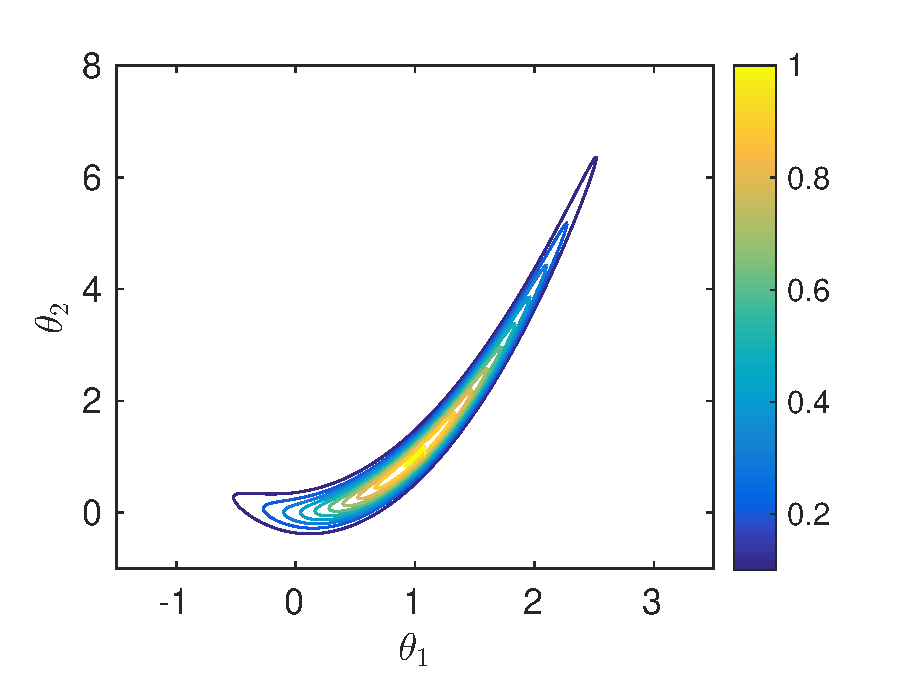
\includegraphics[width=0.31\textwidth]{images/R2_posterior}}
\caption{Visualisation of the density of example $R_1$, as given in Equation~\eqref{eqn:R2_repeat}.}
\label{fig:R2_posterior}
\end{figure}

\subsection{Implementation details}

We now demonstrate some properties of the transport maps we will be using in our MCMC algorithms. We draw 1 million samples from the density in \eqref{eqn:R2_repeat}, and use this sample in the framework of Section~\ref{sec:transport_implementation} to build a transport map. We use this map to push forward the original sample onto the reference space, where we will be able to see how well the map has performed at converting the original sample to a standard Gaussian. We then pull the sample back on to target space using the inverse map to check that our map is invertible and well behaved.

For this example, we use an index set of total order 3 with monomial basis functions. This results in a map of the form
\[
	T(\theta_1, \theta_2) = \begin{bmatrix} T_1(\theta_1) \\ T_2(\theta_1, \theta_2) \end{bmatrix},
\]
where
\begin{align*}
		T_1(\theta_1) &= \gamma_{1,1} + \gamma_{1,2}\theta_1 + \gamma_{1,3}\theta_1^2 + \gamma_{1,4}\theta_1^3, \\
		T_2(\theta_1, \theta_2) &= \gamma_{2,1} + \gamma_{2,2}\theta_1 + \gamma_{2,3}\theta_1^2 + \gamma_{2,4}\theta_1^3
					+ \gamma_{2,5}\theta_2 + \gamma_{2,6}\theta_1\theta_2 \\
				 & \qquad \quad + \gamma_{2,7}\theta_1^2\theta_2 + \gamma_{2,8}\theta_2^2 + \gamma_{2,9}\theta_1\theta_2^2 +
					 \gamma_{2,10}\theta_2^3.
\end{align*}
Clearly even with only basis functions of total order 3, we have a large number of unknowns in our optimisation problem, $\bar{\gamma} \in \mathbb{R}^{14}$. If we were to increase the dimension of $\theta$ further we would need to reduce the number of terms we include in the expansion by, for example, removing all the cross terms. This reduces the quality of our map but since we only require an approximate map we can afford to reduce the accuracy.

\begin{figure}[htpb]
\centering
\subfigure[Original sample $\theta$ from RWMH algorithm.]{\includegraphics[width=0.31\textwidth]{"images/R2_transport_orig"}}\quad
\subfigure[Push forward of $\theta$ onto reference space.]{\includegraphics[width=0.31\textwidth]{"images/R2_transport_ref"}}\quad
\subfigure[Pull back of reference sample onto target space.]{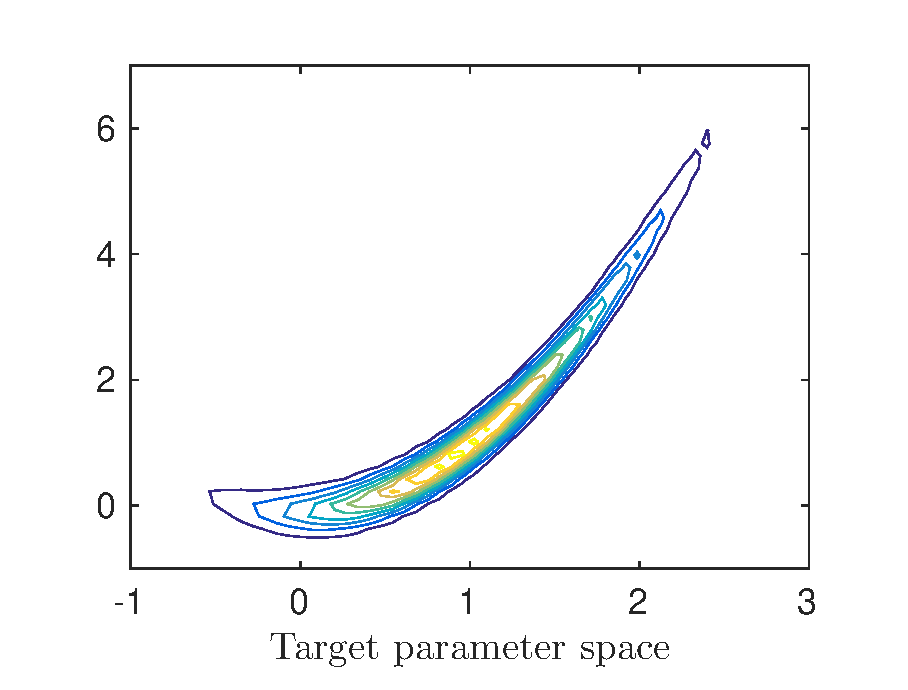
\includegraphics[width=0.31\textwidth]{images/R2_transport_pullback}}
\caption{Rosenbrock target density as described in Equation~\eqref{eqn:R2_repeat}.}
\label{fig:R2_transport}
\end{figure}

Figure~\ref{fig:R2_transport} shows the efficiency of the transport map. Even though we have truncated the infinite expansion in the monomial basis down to 4 and 10 terms in respective dimensions, the push forward of the sample is still a unimodal distribution centred at the origin with standard deviation 1. As you move out into the tails of the reference density more non-Gaussian features form, but these are not too much of a problem when using a suitable proposal distribution. The pullback from reference space, in Figure~\ref{fig:R2_transport}, is an exact match of the original sample since we have not perturbed the sample in reference space. This inversion is well defined in the sampling region, although not necessarily outside.

\begin{figure}[!h]
\centering
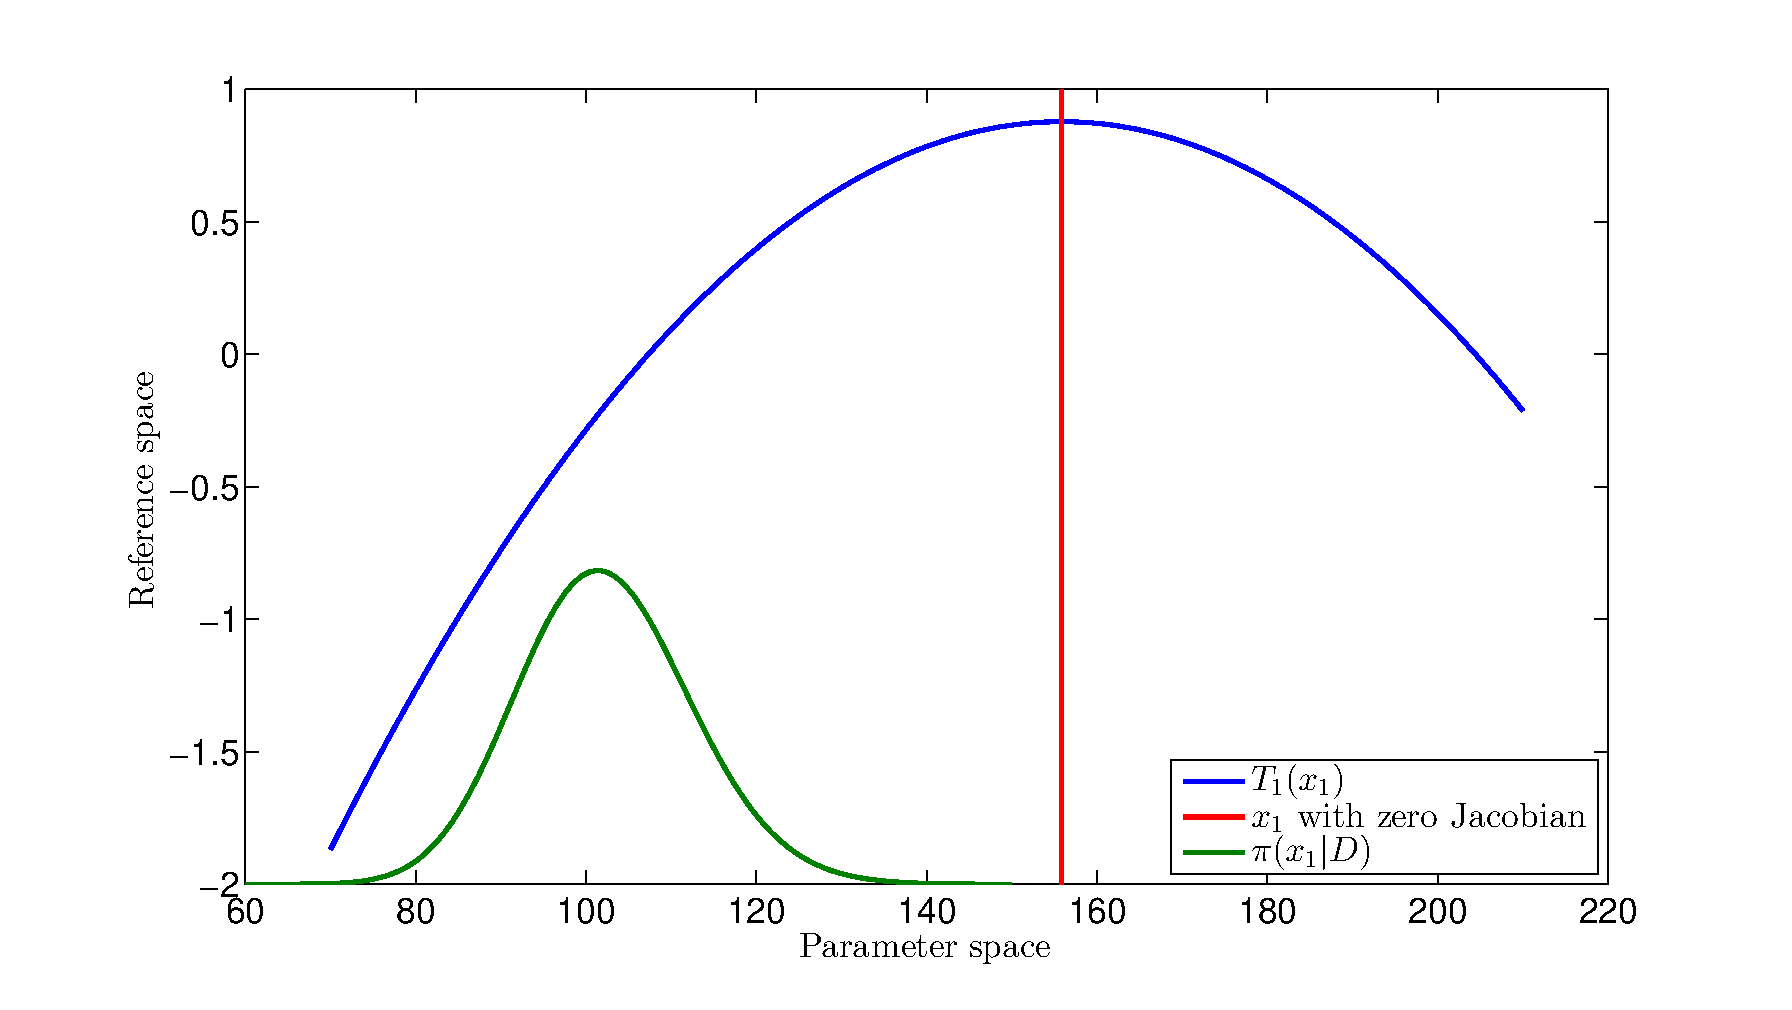
\includegraphics[width=0.8\textwidth]{images/zero_jacobian}
\caption{An example transport map which does not allow exploration of the full target distribution, and has a non-invertible point.}
\label{fig:TM_zero_jacobian}
\end{figure}

If we consider a map built from polynomials of total order $p=2$, it is clear that the map $\tilde{T}$ does not map onto $\mathbb{R}^d$, but on to a subset of it. Figure~\ref{fig:TM_zero_jacobian} illustrates this point. We see that in this dimension, the $\tilde{T}^{-1}$ will not map any proposal $r > 0.8$ to a point in the target space. The point at which no inverse exists for a point $r_1$ can be made arbitrarily far out in the tails of the posterior distribution, but will be finite. The point at which the Jacobian is zero is also a non-invertible point since the logarithm in the pullback becomes infinite. This means that (1) we will never sample from the tail of the target distribution which lies beyond this turning point, and (2) all points in reference space $r < 0.8$ have the possibility of being mapped to two distinct points in target space. We can choose to truncate our parameter space at this turning point which allows our map to be bijective, however we will not be able to sample from the true posterior. For this reason it is best to chose an index set where the maximum order is an odd number.

\subsection[Numerical results]{Numerical results for convergence of transport map based algorithms}

We first find the optimal scaling parameters for the individual algorithms. This is done as before by optimising the effective sample size in the PAIS algorithm, and by tuning the relative $L^2$ error in the MH algorithm. There is currently no guidance on the best way of tuning the MH algorithm with transport map proposals although one might expect results similar to the standard MH results. As in the PAIS algorithm, the effective sample size might be the best option.

\begin{table}[!h]
\centering
\begin{tabular}{lrrr}
\toprule
	Statistic \quad / \quad Algorithm & \ref{alg:TransportMH} & \ref{alg:TransportPAIS1} & \ref{alg:TransportPAIS2}  \\ \cmidrule(lr){1-4}
	$\delta_{L^2}$				 & 1.0e-0 & 1.1e-1 & 3.5e-1 \\
	$\delta_{\text{ESS}}$				 & - & 1.0e-1 & 5.2e-1 \\ \cmidrule(lr){1-4}
	Acc. rate							 & 0.23 & - & - \\
	ESS ratio							 & - & 0.62 & 0.71 \\
\bottomrule
\end{tabular}
\caption{Optimal scaling parameters for the transport map based algorithms applied to $R_1$.}
\label{tab:R2_opt_scaling}
\end{table}

The optimal scaling parameters are given in Table~\ref{tab:R2_opt_scaling}. Here we see that the effective sample size is much lower than we see in the one-dimensional examples with the PAIS algorithms. However, in $R_1$ we are dealing with a much more complicated correlation structure, as well as a very slowly decaying tail in $\theta_2$. We have seen in Section~\ref{sec:LPAIS_R1} that the standard PAIS-RW required an ensemble size of $M=500$ to overcome the problems in this density, however the transport map transforms the tails to be more like those of a Gaussian which can be approximated well by a smaller ensemble size of $M=150$.

\begin{figure}[!h]
\centering
\subfigure[Comparison of the two Transport PAIS options.]{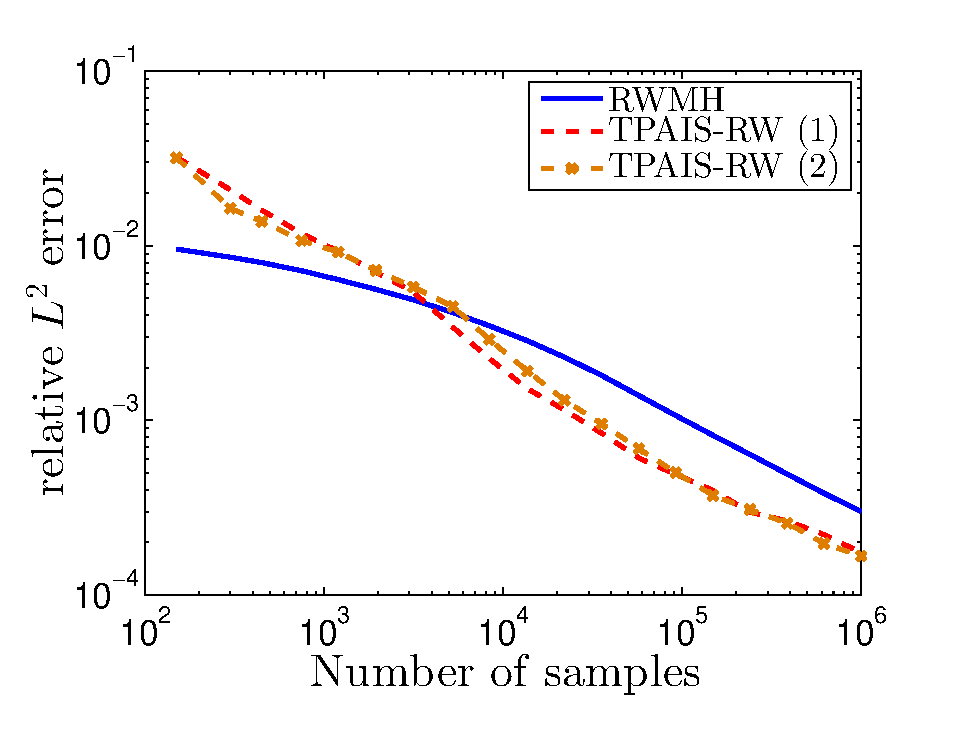
\includegraphics[width=0.45\textwidth]{images/R1_L2}}
\subfigure[Comparison of Transport PAIS option (2) with the standard algorithms.]{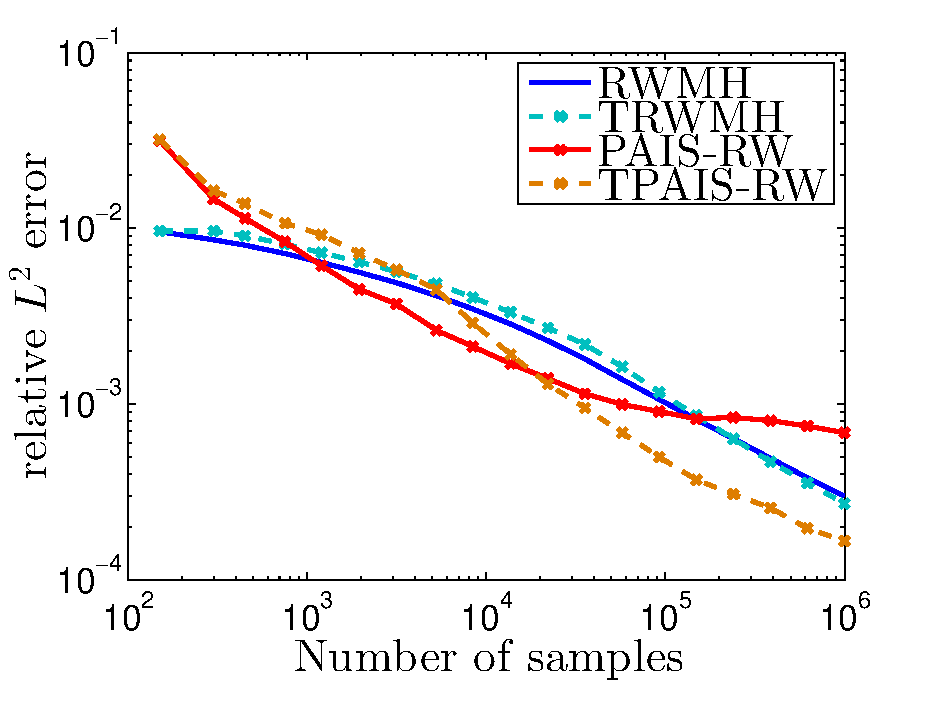
\includegraphics[width=0.45\textwidth]{images/R1_L2_all}}
\caption{Convergence of Algorithms~\ref{alg:TransportMH}, \ref{alg:TransportPAIS1}, \ref{alg:TransportPAIS2} for $R_1$. Ensemble size $M=150$, resampling performed using the AMR algorithm.}
\label{fig:R2_l2_convergence}
\end{figure}

The convergence of the three algorithms is displayed in Figure~\ref{fig:R2_l2_convergence}. Figure (a) shows that the two variations of the transport based PAIS algorithms converge with similar rates. The second version, which performs the resampling stage in reference space rather than target space, has a slightly higher ESS, and is more stable than option (1). This version also has a property that we can exploit in Section~\ref{sec:TPAIS_higher_dim}.

\section{Sampling in higher dimensions}\label{sec:TPAIS_higher_dim}

Algorithm~\ref{alg:TransportPAIS2} allows us to decorrelate the dimensions of our random parameter on reference space, where we then can resample and map the resulting ensemble back onto target space. Since, on reference space, the dimensions are uncorrelated, we are able to resample in each dimension separately. Resampling in a single dimension allows for optimisations in resampling code, and also means that the resampler is not affected by the curse of dimensionality.

If we can approximate the posterior well with our mixture and with the transport map, we should not be affected by the increase in dimension to the extent we have been with the standard PAIS-RW algorithm. In one dimension the ETPF algorithm can be implemented very efficiently. As described in~\cite{reich2013nonparametric}, the coupling matrix has all non-zero entries in a staircase pattern when the state space is ordered. We can exploit this knowledge to produce Algorithm~\ref{alg:ETPF_1d}. Which is much faster than using the simplex algorithm to minimise the associated cost function, and faster than the AMR algorithm.

\begin{table}[!htpb]
\begin{algorithm}[H]
\DontPrintSemicolon
\BlankLine
Sort the states, $\{(w_i, x_i)\}_{i=1}^M$, into ascending order.\;
Normalise the weights $p_i = w_i/\|w\|_1$.\;
Set $y_i \leftarrow 0$ for all $i=1,\dots,M$.\;
Set $c \leftarrow 0$\;
\For{$i \leftarrow 1, \dots, M$}{
	Set $t \leftarrow p_i$\;
	\While{$j \leq M$ and $t > 0$}
	{
		Set $s \leftarrow \left(M^{-1}-c\right) \wedge t$\;
		Increase $y_j$ by $M\times s\times x_i$.\;
		Decrease $t$ by $s$.\;
		Increase $c$ by $s$.\;
		\If{$t>0$}
		{
			Increase $j$ by 1.\;
			Set $c \leftarrow 0$.
		}
	}
}
Return $y$.\;
\caption{ETPF algorithm in one dimension.\label{alg:ETPF_1d}}
\end{algorithm}
\end{table}


\section{Multiscale approximations of likelihoods in stochastic
  reaction networks}\label{sec:multi}

We now move onto our main application area; the modelling of discrete chemical populations and the discovery of reaction rates within these systems. Often when modelling populations of chemical or animal species, the population is large enough that we can consider continuous models, such as coupled differential equations, to describe the evolution of the populations over time. However, this approximation is not always appropriate. These continuous models, when applied to smaller populations, result in time points where there are fractional numbers of a species. In the real world there can only be an integer number of individuals, and the effect on other species in the system might be very different to the continuous model's prediction. It is instead more appropriate to model these systems with stochastic simulation algorithms (SSAs) which model population counts as non-negative integers and take account of the intrinsic noise. The most common SSA is the Gillespie algorithm proposed in 1977~\cite{gillespie1977exact}.

\subsection{Stochastic Simulation Algorithms}\label{sec:SSAs}

SSAs are a powerful tool for describing the dynamics of discrete systems, most commonly used in the description of small scale chemical systems such as in cell biology. These algorithms simulate reactions between different species. A reaction has occurred whenever the populations of the different species in the system change. For example, a simple reaction where two chemicals from the same species join together to form a chemical from a different species, this is denoted
\begin{equation}\label{eqn:chem_reaction}
	X_1 + X_1 \into^{k} X_2
\end{equation}
where the variable $k$ is the rate at which the reaction occurs. These reactions are considered to occur instantaneously. By randomly sampling the time between reactions as well as which reactions occur we can simulate a potential trajectory for the population of a species during a given time interval. Methods for the simulation of these systems assume that the system is in thermal equilibrium and that the density of each species is constant across the entire system domain.

\begin{dfn}[Stochastically exact SSA]
An SSA for a quantity $S_t$ is stochastically exact if at every time point, $t$, the probability that a particular trajectory, $T_t$, takes a value $s$ is equal to the probability of the quantity $S_t$ taking that value, i.e.
\[
	\mathbb{P}(S_t = s) = \mathbb{P}(T_t = s)\quad \forall t \ \text{and} \ s.
\]
At the time $t$, the distribution of $S_t$ is denoted as $\mu_t$.
\end{dfn}
If an SSA is stochastically exact, these trajectories can be used to estimate probability distributions for the population of a species. Empirical distributions for the value of $S_t$ throughout a time interval can be produced by a sufficiently large number of simulated trajectories.

Population models can contain several sources of variability. Large scale heterogeneity such as genetic diversity and environmental factors are often ignored in deterministic modelling. On a smaller scale the population has intrinsic noise which can come from thermal fluctuations at the molecular level~\cite{szekely2014stochastic,mcadams1999sa}. This small scale variability is inherently incorporated into the model dynamics of an SSA, whereas genetic and environmental factors are not. During the time span of a model simulation, we can assume that the genetic factors are constant and, if necessary, environmental factors can be explicitly included by evolving the probabilities of which reactions occur~\cite{shahrezaei2008colored}.

We now describe some methods of approximating $\mu_t$~\cite{gillespie1991markov}. The deterministic master equation is a system of DEs which defines a chemical system, when it is possible to solve this system of differential equations (DEs) we can obtain an exact form for $\mu_t$~\cite{anderson2016product,jahnke2007solving,anderson2010product}. However analytic solutions are rare and it is common to approximate $\mu_t$ using stochastic methods, such as the Gillespie SSA~\cite{gillespie1977exact}, $\tau$-leap methods~\cite{cao2006efficient,cao2005avoiding,chatterjee2005binomial} or SDEs such as the chemical Langevin equation~\cite{gillespie2000chemical}.

%%% Gillespie SSA

The Gillespie algorithm is an example of an exact SSA. The problem is formulated as a set of all possible reactions of the type in Equation~\eqref{eqn:chem_reaction}, the choice of which reaction and when it occurs is decided by a pair of random numbers whose distribution is determined by the relative densities of the chemical species.

\begin{dfn}[Propensity function]
Given $n$ chemical species with populations
\[
	\mathbf{X}(t) = [X_1(t),\dots,X_n(t)]^\top,
\]
the likelihood of a reaction, $R_i$, occurring is determined by the \emph{propensity function}
\[
	\alpha_i(\mathbf{X}(t); \mathbf{k}) = \lim\limits_{\Delta t\rightarrow 0} \! \frac{\mathbb{P}(\text{Reaction $i$ occurs in $[t, t+\Delta t)$})}{\Delta t}
\]
which depends on the current state of the system and the reaction rates $\mathbf{k}$.
\end{dfn}

The propensity function also takes into account the volume of the domain, the temperature, and many other factors. These functions $\alpha_i(\mathbf{X}(t);\mathbf{k})$ are normalised to give the probabilities, $p_i(\mathbf{X}(t);\mathbf{k})$, that $R_i$ will be the next reaction to occur,
\[
	p_i(\mathbf{X}(t); \mathbf{k}) = \frac{\alpha_i(\mathbf{X}(t);\mathbf{k})}{\alpha_0(\mathbf{X}(t);\mathbf{k})}, \quad \text{where} \quad \alpha_0(\mathbf{X}(t);\mathbf{k}) = \sum_i \! \alpha_i(\mathbf{X}(t);\mathbf{k}).
\]
There is a propensity function associated with each of the $d$ possible reactions. The form of these functions is dependent on the type of reaction which occurs. This notation can become cumbersome and so the dependence on the current state and reaction rates may be omitted. The normalisation constant $\alpha_0$ is known as the \emph{total system propensity} or \emph{total propensity}.

The Gillespie algorithm is a stochastically exact algorithm which simulates a Markov jump process about the chemical population state space. The algorithm assumes that reactions occur in intervals which follow an exponential distribution. The rate associated with this exponential distribution is linked to the total system propensity $\alpha_0$. Which reaction occurs at each of these times depends on the distribution $\mathbf{p} = [p_1, \dots, p_d]^\top$.

Simulating a trajectory by sampling every reaction in this way allows us to generate stochastically exact draws from the true distribution $(\mu_t, \forall t)$, however it can be extremely costly, especially when reactions occur on different timescales. Variations on the algorithm have been proposed which reduce the computational cost, these are described in the review \cite{gillespie2007stochastic}.

\begin{table}[!htpb]
\centering
\begin{algorithm}[H]
\DontPrintSemicolon
\BlankLine
	Choose $\mathbf{X}(0) = [x_1, \ldots, x_n]^\top$.\;
	Define $\mathbf{k} = [k_1, \ldots, k_d]^\top$.\;
	Set $j= 0,\ t_0 = 0$.\;
	\While{$t_j < \tau$}{
		Update $\alpha_i(\mathbf{X}(t_j);\mathbf{k})$, for $i=1,\ldots, d$.\;
		Set $\alpha_0 = \sum_i \alpha_i(\mathbf{X}(t_j); \mathbf{k})$ and calculate $\mathbf{p}$.\;
		Sample $\Delta t \sim \text{Exp}(\alpha_0)$ and $r(t_j+\Delta t) \sim \text{Multinomial}(1, \mathbf{p})$.\;
		Set $t_{j+1} \leftarrow t_j + \Delta t$.\;
		Update populations $\mathbf{X}(t_{j+1}) = \mathbf{X}(t_j) + \nu_{r(t_{j+1})}$.\;
		$j \leftarrow j+1$.\;
	}
\caption{The Gillespie Algorithm~\cite{gillespie2007stochastic}.\label{alg:gillespie}}
\end{algorithm}
\end{table}

The Gillespie algorithm is outlined in Algorithm~\ref{alg:gillespie}. At each iteration we calculate the propensities, $\alpha_i(\mathbf{X}(t_j);\mathbf{k})$, based on the current state of each of the populations. We use these propensities to calculate $\alpha_0$ as well as the probabilities, $\mathbf{p}(\mathbf{X}(t_j); \mathbf{k})$. We now generate two random numbers, the first, $r(t_j)$, is from the multinomial distribution defined by the probability vector $\mathbf{p}$, which tells us which reaction occurs next. The second, $\Delta t$, is from the exponential distribution with rate $\alpha_0$, and tells us how long until this reaction occurs. Finally we update the system's state, $\mathbf{X}(t_{j+1})$, according to which reaction has occurred, using the reaction state change vector, $\nu_i$.

\begin{dfn}[State change vectors and the stoichiometric matrix]
	The {\it state change vector} of a reaction $R_i$ is the vector, $\nu_i$, where the $j$th entry corresponds to the change made to the $j$th species by the reaction $R_i$. e.g. In a system with two chemicals $\mathbf{X} = [X_1, X_2]^\top$, and a reaction $R_1\colon X_1 \rightarrow X_2$, the state change vector of $R_1$ is $v_1 = [-1, 1]^\top$. The columns of the {\it stoichiometric matrix} are formed by the state change vectors for each reaction.
\end{dfn}

%%% Multiscale

In many chemical systems, we can find variables which change on more than one time scale. These variables might be a single species, or a linear combination of different species. It is often possible to isolate which variables are changing more frequently (the \textit{fast variables}) and those which are changing less frequently (the \textit{slow variables}). In many cases we are interested in the dynamics of the slow variables, and the full simulation of the fast variables can be considered a waste of computational resources. In real world experiments it can also be difficult to measure the quantities of the fast variables given the relatively short times the system stays in a single state. In this thesis we consider two separate simplifying approaches for these multiscale systems. The first approach uses the quasi-equilibrium assumption.

\begin{dfn}[Quasi-equilibrium assumption]
	The quasi-equilibrium assumption (QEA) is the assumption that the fast variables converge in distribution on a timescale which is negligible with respect to the rate of change of the slow variables.
\end{dfn}

This assumption allows us to approximate the dynamics of the slowly changing quantities in the system by assuming that the fast quantities are in equilibrium with respect to the fast variables in isolation, i.e. the slow rates $\rightarrow 0$. We also consider the constrained multiscale approach (CMA) described in \cite{cotter2011constrained,cotter2016constrained}. The CMA is similar to the QEA except that it takes into account changes in the slow variables which also change the fast variables. We briefly define the CMA as is given in \cite{cotter2016constrained}.

\begin{dfn}[Constrained Projector]\label{dfn:constrained_projector}
	Given a partition of the state space with $N$ variables into $N_s$ slow variables $\mathbf{S} = [S_1,\dots, S_{N_s}]$ and $N_f$ fast variables $\mathbf{F} = [F_1,\dots, F_{N_f}]$. A constrained projector $\mathcal{P}_\mathbf{S}\colon\mathbb{N}^N_0\rightarrow\mathbb{N}^N_0$ maps the values of the slow variables to a given value $\mathbf{S}$, while preserving the values of the fast variables.
\[
	\mathcal{P}_\mathbf{S}([\hat{\mathbf{S}}, \hat{\mathbf{F}}]) = [\mathbf{S}, \hat{\mathbf{F}}], \quad \forall \, [\mathbf{S},\mathbf{F}] \in \mathbb{N}_0^N.
\]
\end{dfn}

\begin{dfn}[Constrained Stoichiometric Projector]
	Given the partition in Definition~\ref{dfn:constrained_projector}, the constrained stoichiometric projector $\mathcal{P}\colon\mathbb{N}_0^{N}\rightarrow\mathbb{N}_0^{N}$ maps all non-zero values of the slow variables to zero.
\[
	\mathcal{P}([\mathbf{S}, \mathbf{F}]) = [\mathbf{0}, \mathbf{F}], \quad \forall \, [\mathbf{S}, \mathbf{F}] \in \mathbb{N}_0^{N}.
\]
\end{dfn}

\begin{dfn}[Constrained subsystem]
	The constrained subsystem is defined for a chemical reaction system, such as those we have been discussing so far, and is the system which arises from partitioning this chemical reaction system as in Definition~\ref{dfn:constrained_projector} and applying the constrained projector, $\mathcal{P}_\mathbf{S}$ to the state vector $\mathbf{X} = [\mathbf{S}, \mathbf{F}]$ after every new reaction, or equivalently applying the constrained stoichiometric projector, $\mathcal{P}$, to the change in state resulting from each reaction. When a stoichiometric vector becomes null by application of $\mathcal{P}$, that reaction can be removed from the system. If a reaction with one of the new stoichiometries would result in a species with a negative population, the propensity of this reaction is set to zero.
\end{dfn}

The CMA accounts for the differences in the invariant distribution of the fast species which are due to the occurrence of slow reactions. When the fast and slow subsystems operate on very different timescales, the CMA and QEA produce near identical results, however when the systems are not so clearly separated the CMA provides superior accuracy. 

In this section we are interested in chemical systems where we have a small number of chemical species. We assume that we have thermal equilibrium and that the chemicals are well mixed so that we have a homogeneous system. We assume that we have accurate observations of the populations of the chemicals and the times of the reactions, and we are concerned with recovering the probability distribution which describes the rates of the reactions. The posteriors arising from situations such as these often have non-Gaussian tails which, as discussed in previous chapters, can cause problems when using kernel density estimations of the posterior distribution as we do in the standard PAIS algorithm. The dynamics of these systems are also highly non-linear resulting in complex correlation structures between parameters.

%%%

\subsection{Sufficient Statistics for Rate Recovery}

Following the assumptions for the modelling of the stochastic process $\mathbf{X}(t),\ t \in (t_0, \tau]$ outlined in the previous section, we can determine sufficient statistics for the probability distributions of the model parameters $\mathbf{k}$. Here we treat the problem in the Bayesian context and so we define a posterior distribution, $\pi(\mathbf{k}|D)$, which incorporates the model likelihoods with prior information for these reaction rates. The data, $D$, is a complete trajectory of a molecular system which includes the times of each reaction as well as which reaction occurs. In practice it might not be obvious which reaction has occurred just by looking at the changes in chemical populations, however we ignore this problem for now.

For a problem with $n$ chemical species, $X_i$,  and $d$ reactions, $R_j$, the data, $D$, has the form given in Table~\ref{tab:chem_data}. The data is measured over a time interval which contains $M$ reactions. We assume that the times between reactions have the exponential distribution, so we define the differences $\Delta t_j = t_{j}-t_{j-1} \sim \text{Exp}\left(\alpha_0(\mathbf{X}(t_{j-1});\mathbf{k})\right)$.

\begin{table}[!h]
\centering
\begin{tabular}{l|r|r|r|}
	\hhline{~|--|}
	Data $D$ \quad & Time & Reaction \\ \hhline{~|=|=|}
	& $t_1$	& $r(t_1)$ \\
	& $t_2$	& $r(t_2)$ \\
	& \vdots & \vdots \\
	& $t_M$	& $r(t_M)$ \\ \hhline{~|--|}
 \end{tabular}
\caption{Form of the data $D$, in the notation given in Algorithm~\ref{alg:gillespie}. The initial time $t_0$ is set to 0.}
\label{tab:chem_data}
\end{table}

At a time $t_j$, the reaction $R_i$ occurs with probability $p_i(\mathbf{X}(t_{j-1});\mathbf{k})$, where the propensities are calculated using the system state at the previous time step,
\[
	r(t_j) \sim \text{Multinomial}\left(1, \mathbf{p}(\mathbf{X}(t_{j-1});\mathbf{k})\right)
\]
All the possible states of the process, $\mathbf{X}(t),\ t \in (t_0,\tau]$, belong in the state space $\mathcal{S}$, the space itself does not depend on time for the problems which we are considering.

From this formulation, we see that the random variables $(\Delta t_j, r(t_j))$ only depend on the states $\mathbf{X}(t_{j-1})$ and so are Markovian. This conditional independence means that we can group events together by what state the system was in when the event happened. We define two new random variables which depend on a state $\mathbf{Y} \in \mathcal{S}$, first the total time spent in state $\mathbf{Y}$,
\[
	T(\mathbf{Y}) = \sum\limits_{j=1}^M \Delta t_j\; \text{I}(\mathbf{X}(t_{j-1}) = \mathbf{Y}).
\]
This random variable, $T(\mathbf{Y})$, is a sum of Exponential distributions, each with the rate $\alpha_0(\mathbf{Y};\mathbf{k})$, and hence follows the Gamma distribution,
\begin{equation}\label{eqn:chem_time_dist}
	T(\mathbf{Y}) \sim \text{Gamma}\left(\alpha=K(\mathbf{Y}),~\beta = \alpha_0(\mathbf{Y}; \mathbf{k})\right),
\end{equation}
where $K(\mathbf{Y}) = \sum\limits_{j=1}^M \text{I}(\mathbf{X}(t_{j-1}) = \mathbf{Y})$.

Similarly, we can define the reactions which occurred when the system was in state $\mathbf{Y}$ as $\mathbf{r}(\mathbf{Y}) = [r_1(\mathbf{Y}), \ldots, r_d(\mathbf{Y})]^\top$ where
\[
	r_i(\mathbf{Y}) = \sum\limits_{j=1}^M \text{I}(r(t_j) = i \textbf{ and }\mathbf{X}(t_{j-1}) = \mathbf{Y}).
\]
Here all the random variables $r(t_j)$ follow the same multinomial distribution, and so
\begin{equation}\label{eqn:chem_react_dist}
	\mathbf{r}(\mathbf{Y}) \sim \text{Multinomial}(K(\mathbf{Y}),~\mathbf{p}(\mathbf{Y})). 
\end{equation}
The random variables defined in Equations~\eqref{eqn:chem_time_dist} and \eqref{eqn:chem_react_dist} are sufficient statistics for the posterior distribution $\pi(\mathbf{k}|D)$. With these definitions we define two new structures
\[
	\mathbf{T} = [T(\mathbf{Y}_1), \dots, T(\mathbf{Y}_K)]^\top, \quad \text{and} \quad \mathbf{R} = [\mathbf{r}(\mathbf{Y}_1), \dots, \mathbf{r}(\mathbf{Y}_K)]^\top,
\]
where $K = |\mathcal{S}|$, the number of states in $\mathcal{S}$, and each state $\mathbf{Y}_i \in \mathcal{S}$ has been enumerated. We use these structures to define shorter notation,
\[
	\mathbf{T}_i = T(\mathbf{Y}_i), \quad \mathbf{R}_{ij} = r_j(\mathbf{Y}_i), \quad \text{and} \quad \mathbf{K}_i = K(\mathbf{Y}_i).
\]

\subsection{Posterior Distribution}\label{sec:chem_stoch_posterior}

To construct the posterior distribution for the reaction rates, $\mathbf{k}$, in the chemical system, we formulate the likelihood using the sufficient statistics derived in the previous section. Due to the positivity of these reaction rates, we assign a Gamma prior distribution to each rate. Given the distributions in Equations~\eqref{eqn:chem_time_dist} and~\eqref{eqn:chem_react_dist} for our data, the likelihood of observing the data $\mathbf{R}$ and $\mathbf{T}$ is
\[
	\ell(\mathbf{R}, \mathbf{T}|\mathbf{k}) \propto \prod\limits_{i=1}^K \text{Multi}(\mathbf{r}(\mathbf{Y}_i); \mathbf{K}_i, \mathbf{p}(\mathbf{Y}_i))\text{Gamma}(\mathbf{T}_i; \mathbf{K}_i, \alpha_0(\mathbf{Y}_i)),
\]
where again $\mathbf{Y}_i \in \mathcal{S}$ and the propensities $\alpha_i$ and probabilities $p_i$ depend on the reaction rates $\mathbf{k}$.

Our choice of Gamma prior distributions with hyper-parameters $(a_i, b_i)$ results in the posterior distribution of the form
\begin{align}
	\pi(\mathbf{k}|\mathbf{R}, \mathbf{T}) &\propto \ell(\mathbf{R}, \mathbf{T}|\mathbf{k})
	\prod_{i=1}^d \! \text{Gamma}(k_i; a_i, b_i) \notag \\
		&\propto \exp\Bigg\{\sum\limits_{i=1}^K \Bigg[
				\mathbf{K}_i\log \alpha_0(\mathbf{Y}_i; \mathbf{k}) - \mathbf{T}_i\alpha_0(\mathbf{Y}_i; \mathbf{k}) %\notag \\
%		& \qquad\qquad\qquad
				+\sum_{j=1}^d \mathbf{R}_{ij}\log\mathbf{p}_j(\mathbf{Y}_i; \mathbf{k})
			\Bigg]  \notag\\
		&	\qquad\qquad\qquad{} + \sum_{i=1}^d ((a_i-1)\log k_i - b_ik_i)\Bigg\}. \label{eqn:chem_posterior}
\end{align}

\section{Mono-molecular examples}

In this section we look at two examples of chemical systems to demonstrate the effectiveness of the Bayesian approach. These two systems will only contain mono-molecular reactions, i.e. reactions which convert one species into another species at a particular rate. As shown in~\cite{anderson2010product} these systems have a Poisson invariant distributions on the populations. In the limit of infinite reactions, a mono-molecular reaction system with $n$ species will follow the distribution
\begin{equation}\label{eqn:mono_stat_dist}
	\mathbb{P}(X_1=x_1, \ldots, X_n=x_n) = \left(\prod_{i=1}^n \! \frac{\bar{c}_i^{x_i}}{x_i!}\right)\exp\left(-\sum_i^n \! \bar{c}_i\right),
\end{equation}
where $x_i \in \mathbb{N}$ and $\bar{c}_i$ are the complex balances or the concentration of chemical $X_i$ according to the solution of a steady state approximation of the system. We make use of this distribution to formulate posteriors for the chemical reaction rates using the constrained multiscale approach, as in~\cite{cotter2016constrained}.

%%%%%

\subsection{A Multiscale Chemical System}\label{sec:chem_multiscale}

In this section, we consider a simple multiscale example involving two chemical species $S_1$ and $S_2$:
\begin{equation}\label{eqn:full_system}
	\emptyset \xrightarrow{k_1} S_1 \xleftrightarrows[k_3]{k_2} S_2 \xrightarrow{k_4} \emptyset.
\end{equation}
Each arrow represents a reaction from a reactant to a product, with
some rate constant $k_i$, and where the rates of the reactions are
assumed to follow mass action kinetics. The parameters $k_i$ are strictly positive, and $\mathbf{k} = [k_1,\dots,k_4]^\top \in \mathbb{R}_+^4 = \mathcal{X}$. We denote the concentration of
species $S_i$ by $X_i$. We assume that we are in a
parameter regime such that the reactions $R_2\colon S_1\rightarrow S_2$ and $R_3\colon S_2\rightarrow S_1$ occur
more frequently than the other reactions, $R_1\colon \emptyset \rightarrow S_1$, and $R_4\colon S_2 \rightarrow \emptyset$. Notice that both
chemical species are involved in fast reactions. However, the quantity
$X = X_1 + X_2$, corresponding to an artificial species $S$, is conserved by both of the fast reactions,
and as such, this is the slowly changing quantity in this system.
When recording our data, we are only able to take readings of the reactions which change the slow variable $S$. 
The effective dynamics of $S$ can be represented as follows
\begin{equation}\label{eqn:QSSA_system}
	\emptyset \xrightarrow{k_1} S \xrightarrow{\hat{k}_4} \emptyset.
\end{equation}
The new reaction rate $\hat{k}_4$ is approximated through
application of the two approaches mentioned in Section~\ref{sec:SSAs}. Under the QEA, the value of $\mathbb{E}\left[k_4X_2|S=s\right]$ is found by computing the invariant distribution of the fast subsystem of reactions~\cite{jahnke2007solving},
\[
	S_1 \xleftrightarrows[k_3]{k_2} S_2, \qquad X_1 + X_2 = s
\]
which tells us that $X_2$ is distributed according to Bin$(S, k_3(k_3+k_4)^{-1})$ and so
\[
	\hat{k}_4^{\text{QEA}}(s) = \mathbb{E}_{\text{QEA}}\left[k_4X_2|S=s\right] = \frac{k_2k_4s}{k_2+k_3}.
\]
Similarly, the analysis of the constrained system as discussed in~\cite{cotter2016constrained} yields the effective propensity
\begin{equation}\label{eqn:chem_CMA_rate}
	\hat{k}_4^{\text{CMA}}(s) = \mathbb{E}_{\text{CMA}}\left[k_4X_2|S=s\right] = \frac{k_2k_4s}{k_2+k_3+k_4}.
\end{equation}

Our observations are uninformative about the reaction rates $k_2, k_3$, and $k_4$, as there
is a sub-manifold $\mathcal{M} \subset \mathcal{X}$ along which the effective rate
$\hat{k}_4$ is invariant, leading to a highly ill-posed inverse
problem. This type of problem is notoriously difficult to
sample from using standard MH algorithms, as the algorithms quickly
find a point on $\mathcal{M}$ but then
exploration around $\mathcal{M}$ is slow.

\subsubsection{Target Distribution}\label{sec:multiscale_posterior}

We can use the posterior distribution derived in Section~\ref{sec:chem_stoch_posterior} to specify the posterior distribution for each of the three scenarios we are interested in. We would like to find out how the posterior distributions we obtain from the two models, the QEA and CMA, differ to the posterior for a complete data set.

In all three cases, we find the posterior distribution for $\mathbf{k} \in \mathcal{X}$. These four parameters are assigned Gamma prior distributions,
\[
	k_i \sim \text{Gamma}(\cdot; \alpha_i, \beta_i), \quad \text{for} \quad i = 1, \dots, 4.
\]
The hyper-parameters corresponding to each of these prior distributions are given in Table~\ref{tab:multiscale_priors}. These priors are the same for each of the three posterior distributions.

\begin{table}
\centering
\begin{tabular}{|l|R{2em}R{2em}R{2em}R{2em}|}
	\hline
	parameter/dimension & 1 & 2 & 3 & 4 \\ \hline
	$\alpha_i$ & 150 & 5 & 5 & 3 \\
	$\beta_i$ & 15/9 & 5/12 & 5/12 & 1 \\ \hline
\end{tabular}
\caption{Hyper-parameters in the prior distributions for the multiscale problem described in Section~\ref{sec:multiscale_posterior}.}
\label{tab:multiscale_priors}
\end{table}

Under the QEA and CMA simplifications, we reduce the information contained in the data, as defined in Table~\ref{tab:chem_data}. We now only have one species, $S$, and two reactions,
\[
	R_1\colon \emptyset \xrightarrow{k_1} S, \quad \text{and} \quad R_2\colon S \xrightarrow{\hat{k}_4} \emptyset,
\]
hence the state space of our system is much smaller. This means it is much faster to evaluate the posterior given in Equation~\eqref{eqn:chem_posterior}. For the full data scenario, the dimension of the parameter $\mathbf{k}$ is $d$ and we have $d$ reactions, however when using the QEA or CMA simplifications, the number of reactions is reduced to $n=2$ so that $d \neq n$. i.e. We slightly modify the posterior from Equation~\eqref{eqn:chem_posterior} to
\begin{align}
	\pi(\mathbf{k}|\mathbf{R}, \mathbf{T}) &\propto \exp\Bigg\{\sum\limits_{i=1}^K \Bigg[
				\mathbf{K}_i\log \alpha_0(\mathbf{Y}_i; \mathbf{k}) - \mathbf{T}_i\alpha_0(\mathbf{Y}_i; \mathbf{k})
				+\sum_{j=1}^{n} \mathbf{R}_{ij}\log\mathbf{p}_j(\mathbf{Y}_i; \mathbf{k})
			\Bigg]  \notag\\
		&	\qquad\qquad\qquad{} + \sum_{i=1}^d ((a_i-1)\log k_i - b_ik_i)\Bigg\}, \label{eqn:chem_QEA_posterior}
\end{align}
where $n=4$ for the full data model, and $n=2$ for the simplifications.

\begin{figure}[htb]
\centering
\includegraphics[width=0.9\textwidth]{"images/CMA_posterior"}
\caption{Posterior for the constrained multiscale problem outlined in Section~\ref{sec:chem_multiscale}.}
\label{fig:chem_CMA_posterior}
\end{figure}

Figure~\ref{fig:chem_CMA_posterior} shows how this posterior looks when we use the constrained approach in Equation~\eqref{eqn:chem_CMA_rate} to model the effective degradation rate $\hat{k}_4$.

\subsubsection{Implementation}\label{sec:chem_implementation}

For the posterior distribution in \eqref{eqn:chem_QEA_posterior}, we consider several proposal methods. First we implement both the PAIS and MH algorithms with a Gaussian proposal distribution. In the case of the PAIS algorithm, this is a Gaussian mixture proposal distribution. The proposal distribution uses a covariance matrix which has been constructed using the sample covariance of a sample produced using a standard RWMH algorithm. We also compare the PAIS and MH algorithms when using a transport map proposal distribution. This proposal method was discussed in detail in Chapter~\ref{sec:TransportPAIS}.

\begin{figure}
	\centering
	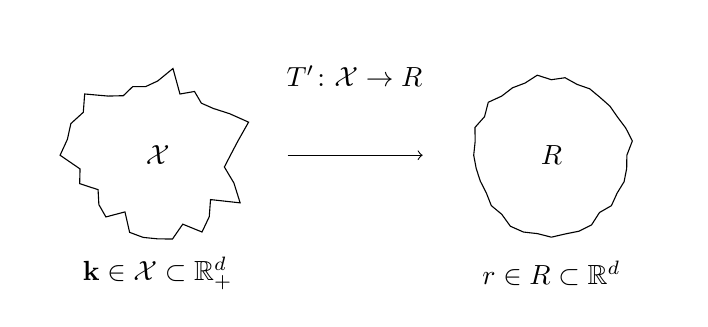
\begin{tikzpicture}
		\pgfmathsetseed{1}

		\node[inner sep=1.5cm,outer sep=0] (A) at (0,0) {$\mathcal{X}$};
		\node[inner sep=1.5cm,outer sep=0] (B) at (5,0) {$R$};

		\draw (A) \irregularcircle{1cm}{2.5mm};
		\draw (B) \irregularcircle{1cm}{0.5mm};

		\draw [->] (A) -- (B);

		\node at (2.5,1) {$T'\colon\mathcal{X}\rightarrow R$};

		\node at (0,-1.5) {$\mathbf{k}\in\mathcal{X}\subset\mathbb{R}_+^d$};
		\node at (5,-1.5) {$r\in R\subset\mathbb{R}^d$};
	\end{tikzpicture}
	\caption{Couplings between parameter space and reference when using the transport map proposal method to propose moves on parameter space.}
	\label{fig:chem_coupling}
\end{figure}

Figure~\ref{fig:chem_coupling} shows how we define a bijective map, $T'$, between parameter space $\mathcal{X}$ and a reference space $R$. In practice we cannot ensure that the approximate map $\tilde{T}'$ is uniquely invertible over the whole of $R$ and so $\tilde{T}'$ is not truly bijective. This leads to problems for our strictly positive state space, $\mathcal{X} \subset \mathbb{R}_+^d$, since proposals in $R$ do not necessarily map back on to $\mathcal{X}$. This motivates the use of a third intermediate space. When using the transport map proposal distribution, we prefix the proposal method with a T, e.g. MH-RW (RWMH) and MH-TRW, as well as PAIS-RW and PAIS-TRW.

We also consider how these algorithms perform when they are applied to the log of the reaction rates. We choose to use this log transformation since it converts our strictly positive parameter space, $\mathcal{X}$, into an intermediate space $\mathcal{Y} \subset \mathbb{R}^d$. This allows us to define $T$ between two subsets of $\mathbb{R}^d$, which means that even if $\tilde{T}$ is not uniquely invertible in some region of $R$, all possibilities are valid proposals. As before, the proposal distributions are labelled with a T for transport map and when using the intermediate space we prepend `log' to the proposal method, e.g. MH-logRW and MH-logTRW, with, PAIS-logRW and PAIS-logTRW.

\begin{figure}
	\centering
	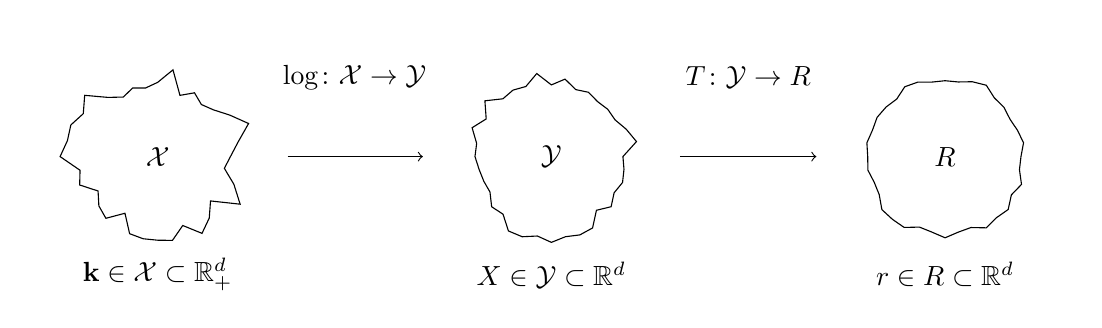
\begin{tikzpicture}
		\pgfmathsetseed{1}

		\node[inner sep=1.5cm,outer sep=0] (A) at (0,0) {$\mathcal{X}$};
		\node[inner sep=1.5cm,outer sep=0] (B) at (5,0) {$\mathcal{Y}$};
		\node[inner sep=1.5cm,outer sep=0] (C) at (10,0) {$R$};

		\draw (A) \irregularcircle{1cm}{2.5mm};
		\draw (B) \irregularcircle{1cm}{1.1mm};
		\draw (C) \irregularcircle{1cm}{0.5mm};

		\draw [->] (A) -- (B);
		\draw [->] (B) -- (C);

		\node at (2.5,1) {$\log\colon\mathcal{X}\rightarrow\mathcal{Y}$};
		\node at (7.5,1) {$T\colon\mathcal{Y}\rightarrow R$};

		\node at (0,-1.5) {$\mathbf{k}\in\mathcal{X}\subset\mathbb{R}_+^d$};
		\node at (5,-1.5) {$X\in\mathcal{Y}\subset\mathbb{R}^d$};
		\node at (10,-1.5) {$r\in R \subset\mathbb{R}^d$};
	\end{tikzpicture}
	\caption{Couplings between parameter space, an intermediate space and reference space when using the transport map proposal method to propose moves on a log space.}
	\label{fig:chem_log_coupling}
\end{figure}

Figure~\ref{fig:chem_log_coupling} displays the composition of maps when we include this intermediate space $\mathcal{Y}$. Every proposal in $R$ results in a valid proposal on $\mathcal{X}$. The inclusion of this additional map means that we must again alter our importance weight definition to reflect the pullback from $R$ through $\mathcal{Y}$. The weight is now
\[
	w_i(\theta') = \frac{\pi(\theta'|\mathbf{R},\mathbf{T})}{Q(\tilde{T}\circ\log(\theta')|\tilde{T}\circ\log(\theta^{(i-1)}))|J_{\tilde{T}\circ\log}(\theta')|},
\]
where $\theta'$ is a proposal on $\mathcal{X}$, $\theta^{(i-1)}$ is the ensemble of states from the previous iteration, and $J_{\tilde{T}\circ\log}(\theta')$ is the Jacobian of the composition of the two maps. This Jacobian is straightforward to calculate,
\[
	|J_{\tilde{T}\circ\log}(\theta')| = |J_{\tilde{T}}(\log(\theta'))||J_{\log}(\theta')|,
\]
where the first determinant is as we saw in the previous chapter, and the second is
\[
	|J_{\log}(\theta')| = \prod\limits_{i=1}^d \frac{1}{\theta'_i}.
\]

% choices made in transport map
For this problem, we continue to use monomials in each dimension in our transport map construction. We use polynomials of total order $p=3$ as the basis functions, i.e.
\[
	T_i(\theta) = \sum_{\mathbf{j}\in\mathcal{J}^{\text{TO}}_i(p)} \gamma_{i,\mathbf{j}}\psi_{\mathbf{j}}(\theta) \quad \text{where} \quad \psi_\mathbf{j}(\theta) = \prod\limits_{k=1}^i \theta_k^{j_k},
\]
and
\[
	\mathcal{J}^{\text{TO}}_i(p) = \{\mathbf{j} \in \mathbb{N}^d_0\ |\ \|\mathbf{j}\|_1 \leq p, \ \text{and}\ j_k = 0\ \forall k > i\}.
\]

% choice of resampler?
As with the mixture model in Section~\ref{sec:app_mixture}, we will use the AMR resampler with an ensemble size of $M=500$. This increase in ensemble size from Chapter~\ref{sec:PAIS} compensates for the increase in parameter dimension.

% analysis method
To measure the convergence of the sampling methods in this section, we will compare the convergence of the mean of each parameter. We approximate $\mathbb{E}(\mathbf{k})$ using 2.4 billion samples from the MH-RW algorithm.

% numerics.
\subsubsection{Convergence Analysis for the Constrained Approach to a Multiscale Chemical Reaction Model}\label{sec:chem_conv}

In this section, we demonstrate the convergence of the sample mean $\hat{\mathbf{k}}$ by approximating the relative error between the sample mean and the true mean $\mathbb{E}(\mathbf{k})$. We do this for each of the eight algorithms introduced in the previous section. Convergence is shown for the constrained approach to the multiscale system, i.e. to the posterior in Equation~\eqref{eqn:chem_QEA_posterior} with the effective degradation rate, $\hat{k}_4^{\text{CMA}}$, from Equation~\eqref{eqn:chem_CMA_rate}.

\begin{table}[!h]
\centering
\begin{tabular}{rrrrrr}
\toprule
	\multicolumn{1}{l}{Algorithm} & \multicolumn{3}{c}{MH} & \multicolumn{2}{c}{PAIS} \\ \cmidrule(lr){2-4} \cmidrule(lr){5-6}
	& & $\delta_\%$ & & $\delta_{\text{ESS}}$ & ESS \\ \midrule
	RW & & 5.5e-3 & & 1.0e-0 & 9.0e-3 \\
	TRW & & 1.2e-0 & & 4.0e-1 & 1.2e-3 \\
	logRW & & 1.7e-1 & & 1.2e-0 & 6.0e-2 \\
	logTRW & & 2.7e-2 & & 1.5e-1 & 3.5e-1 \\
\bottomrule
\end{tabular}
\caption{Optimal scaling parameters for the MH and PAIS algorithms applied to the constrained multiscale problem in Section~\ref{sec:chem_multiscale}. MH parameters optimised by acceptance rate, and PAIS parameters optimised using effective sample size.}
\label{tab:chem_multiscale_scaling}
\end{table}

The optimal scaling parameters are given in Table~\ref{tab:chem_multiscale_scaling}. We note that for MH-TRW and PAIS-TRW the scaling parameter is near to 1, particularly for MH-RW, this is what we should expect since the proposal is made on a reference space which should be near to $\mathcal{N}_d(0, \text{I})$. The same should be true for the MH-logTRW and PAIS-logTRW algorithms since these have the same target reference space, however the optimal scaling parameters here are much smaller. We see that the ESS is higher for the algorithms which sample on $\mathcal{Y}$, and we expect that convergence will be fastest for the PAIS-logTRW algorithm.

\begin{figure}[!htb]
\centering
\subfigure[Sampling algorithms on $\mathcal{X}$.]{\includegraphics[width=0.495\textwidth]{"images/CMA_L2_param_space"}}
\subfigure[Sampling algorithms on $\mathcal{Y}$.]{\includegraphics[width=0.495\textwidth]{"images/CMA_L2_log_space"}}
\caption{Convergence of the constrained multiscale example described in Section~\ref{sec:chem_multiscale}.}
\label{fig:chem_multiscale_L2}
\end{figure}

Convergence of the eight algorithms for this example is shown in Figure~\ref{fig:chem_multiscale_L2}. We first note the poor performance of the MH based algorithms, each of them taking roughly 10,000 samples to begin converging. Only the MH-TRW is at all competitive with the PAIS algorithms. During the simulation interval, the MH-TRW algorithm has not settled down to the expected $\mathcal{O}(1/\sqrt{N})$ rate which means that the estimate is still biased by the long burn-in time. As we have seen in previous examples, the burn-in time for the PAIS algorithm is negligible.

The PAIS variants with RW and TRW proposals perform similarly on both sample spaces. When sampling on $\mathcal{X}$ the transport map is not quite as efficient, largely due to the difficulties discussed in the previous section i.e. many proposals are made which do result in negative reaction rates. Sampling on $\mathcal{Y}$ leads to more comparable Monte Carlo errors, with the logTRW being apparently slightly less stable. This proposal method becomes more stable as we increase either the ensemble size, or the number of iterations between updates of the transport map, $T$. Overall we see the smallest Monte Carlo errors for a given amount of computational effort coming from the PAIS-logTRW algorithm.

\begin{figure}[!htb]
\centering
\subfigure[Reference space mapped to by $T'$.]{\includegraphics[width=0.495\textwidth]{"images/CMA_ref_space_MHTRW"}}
\subfigure[Reference space mapped to by $T\circ\log$.]{\includegraphics[width=0.495\textwidth]{"images/CMA_ref_space_MHlogTRW"}}
\caption{Reference space for the TRW and logTRW proposal distributions. Components are linked by the relation $r_i = T_i'(k_i)$ in (a) and $r_i = T_i\circ\log(k_i)$ in (b).}
\label{fig:chem_reference_spaces}
\end{figure}

We now look at the proposal distributions of the transport map accelerated algorithms. In Figure~\ref{fig:chem_reference_spaces}, we see the reference spaces found by; in (a) mapping the posterior through the map $T'$, and in (b) by mapping the posterior through $T\circ\log$. For the most part, each of these marginal distributions can be recognised as a Gaussian. However, with the exception of $\mathbb{P}(r_2,r_3)$, we would not consider them to be close to a standardised $\mathcal{N}(0, \text{I})$ distribution. Before thinking that the transport map has not helped us to find a `nicer' space on which to propose new values we should consider that the dimensions are now (1) largely uncorrelated, and (2) the variances in each dimension are much more similar than they are in Figure~\ref{fig:chem_CMA_posterior}.

Particularly in Figure~\ref{fig:chem_reference_spaces} (b) we see that $\text{var}(r_1)$ and $\text{var}(r_4)$ are much smaller than $\text{var}(r_2)$ and $\text{var}(r_3)$. To combat this we have a number of choices, we might wish to use two different scaling parameters to match these scales, which would require knowledge of the reference space before beginning sampling. We could alternatively use a proposal distribution such as in the LPAIS algorithm to adaptively learn this at each iteration. Another option is to increase the total order of our index set. For these numerics we have chosen $p=3$, but we know that we can obtain reference spaces which are closer to $\mathcal{N}_d(0, \text{I})$ by choosing a larger $p$.

\subsubsection{Comparison of the Constrained and QEA approaches}

The convergence analysis has been performed for the constrained approach to this multiscale system. We now look at the differences between the constrained and QEA posterior distributions. Recall that the approaches differed only in the form of the effective degradation rate $\hat{k}_4$,
\[
	\hat{k}_4^{\text{QEA}}(s) = \frac{k_2k_4s}{k_2+k_3} \quad \text{and} \quad \hat{k}_4^{\text{CMA}}(s) = \frac{k_2k_4s}{k_2+k_3+k_4}.
\]
This difference in the denominator causes a shift in the parameters as can be seen in Figure~\ref{fig:chem_diff}. The figure shows the difference in posteriors,
\begin{equation}\label{eqn:chem_diff}
	\text{diff}(\mu^{\text{CMA}}, \mu^{\text{QEA}}) = \pi^{\text{CMA}}(\mathbf{k}|\mathbf{R},\mathbf{T}) - \pi^{\text{QEA}}(\mathbf{k}|\mathbf{R},\mathbf{T}).
\end{equation}

\begin{figure}[htb]
\centering
\includegraphics[width=0.9\textwidth]{"images/Diff_CMA_QEA"}
\caption{Difference between the CMA and QEA posteriors as defined in Equation~\eqref{eqn:chem_diff}.}
\label{fig:chem_diff}
\end{figure}

Since the two posteriors have been approximated using an MCMC sample, there is a significant amount of noise, particularly in the tails of the distributions We can see that the differences in the marginals for $k_1, k_2,$ and $k_3$ are relatively small and the differences are largely positive. These positive differences tell us that the constrained approach claims to be more informative about the values of these first three parameters. However the marginal for $k_4$ varies by a significant amount and is more negative. This means that the mean estimates for $k_4$ differ by a large amount, the posterior for the QEA is most peaked.

% compare solution with full data.
We now consider how we should interpret the information given by these models. The QEA assumption tells us that we cannot observe the parameters $k_2$, $k_3$ and $k_4$ independently from the reduced data set, but we can observe the quantity $\hat{k}_4^{\text{QEA}} = k_2k_4/(k_2+k_3)$. Similarly, the constrained approach tells us that we are able to observe the quantity $\hat{k}_4^{\text{CMA}} = k_2k_4/(k_2+k_3+k_4)$. To validate our inferences on $k_2$, $k_3$ and $k_4$ we would like to discover which model is most accurate and informative about these parameters, and which model gives us results which are most similar to what we can obtain from the full model, with all reactions observed.

A conventional way to compare two models under a Bayesian framework is to calculate the Bayes factors~\cite{chen2012monte}. The Bayes factor, $B_{1,2}$, between two models, $\mathcal{M}_1$ and $\mathcal{M}_2$, can be interpreted as a ratio of the normalisation constants of the posterior distributions given each model,
\[
	B_{1,2} = \frac{\mathbb{P}(D|\mathcal{M}_1)}{\mathbb{P}(D|\mathcal{M}_2)}, \quad \text{where} \quad \mathbb{P}(D|\mathcal{M}_k) = \int_\mathcal{X} \mathbb{P}(D|\theta_k,\mathcal{M}_k)\mathbb{P}(\theta_k|\mathcal{M}_k) \, \text{d}\theta_k.
\]
Under the PAIS framework, it is straightforward to calculate these factors using the Monte Carlo estimator for the normalisation constants. From~\cite{robert2013monte} these normalisation constants take the form
\[
	Z_k \approx \hat{Z}_k\frac{1}{NM}\sum_{i=1}^N\sum_{j=1}^M w_j^{(i)}(\mathcal{M}_k),
\]
where $w_j^{(i)}(\mathcal{M}_k)$ is the weight under model $\mathcal{M}_k$ corresponding to the $j$-th ensemble member on the $i$-th iteration. Hence, $B_{1,2} \approx \hat{Z}_1/\hat{Z}_2$. We can compare more than two models in this way by selecting the model with the largest marginal distribution as the best model.

We now label the constrained model as $\mathcal{M}_1$, the model arising from the QEA as $\mathcal{M}_2$, and the full data model as $\mathcal{M}_0$. Under $\mathcal{M}_1$, the parameter $\theta_1 = (k_1, \hat{k}_4^{\text{CMA}})^\top$, and under $\mathcal{M}_2$, the parameter $\theta_2 = (k_1, \hat{k}_4^{\text{QEA}})^\top$. The full model $\mathcal{M}_0$ observes all four parameters $\theta_0 = (k_1, k_2, k_3, k_4)^\top$. The marginal densities for the data, evaluated at the observed data, given the models are displayed in Table~\ref{tab:chem_Bayes_marginals}.

\begin{table}[!htb]
\centering
\begin{tabular}{rr}
	\toprule
	$k$ & \quad $\mathbb{P}(D = (\mathbf{R},\mathbf{T})^\top|\mathcal{M}_k)$ \\ \cmidrule(lr){1-2}
	0 & 6.8e-3 \\
	1 & 3.2e-3 \\
	2 & 1.7e-3 \\ \bottomrule
\end{tabular}
\caption{Marginal distributions for the data $(\mathbf{R},\mathbf{T})^\top$ for each model considered in Section~\ref{sec:multiscale_posterior}.}
\label{tab:chem_Bayes_marginals}
\end{table}

Computing the Bayes factors from Table~\ref{tab:chem_Bayes_marginals} we see that we should of course prefer the model in which we observe all reactions perfectly, however this model is not significantly better than the CMA model ($B_{0,1} = 2.09 < 3.2$, ~\cite{kass1995bayes}). Again the constrained model is not substantially more attractive than the QEA model when we consider the Bayes factor $B_{1,2} = 1.96 < 3.2$. The Bayes factor $B_{0,2} = 4.1 > 3.2$ does tell us that we should significantly prefer the full model to the QEA approximation of the posterior. These Bayes factors present a weak argument that that the constrained model provides us with a better description of the data than the QEA model. We can also present this information graphically, which might provide us with a greater justification for preferring the constrained approximation of the posterior.

\begin{figure}[!htb]
\centering
\subfigure[Marginal for $\hat{k}_4^{\text{QEA}}$.]{\includegraphics[width=0.495\textwidth]{"images/QEA_approx_marginal"}}
\subfigure[Marginal for $\hat{k}_4^{\text{CMA}}$.]{\includegraphics[width=0.495\textwidth]{"images/CMA_approx_marginal"}}
\caption{Comparison of the approximate marginal densities for the `observable parameter' $\hat{k}_4$ under models $\mathcal{M}_1$ and $\mathcal{M}_2$. Marginals for these two parameters are approximated using samples which have been produced by targeting the three densities $\pi_i = \mathbb{P}(\theta_i|D,\mathcal{M}_i)$ for $i = 0, 1, 2$.}
\label{fig:chem_model_comp}
\end{figure}

Figure~\ref{fig:chem_model_comp} displays the marginal distributions for the parameters $\hat{k}_4^{\text{QEA}}$ and $\hat{k}_4^{\text{CMA}}$. For each of these two observable parameters we obtain approximations for three marginal distributions, $\pi_i(\cdot|D, \mathcal{M}_i)$, $i = 0, 1, 2$. Each of these approximations has been produced by marginalising a sample drawn from the full posterior $\pi_i(\mathbf{k}|D, \mathcal{M}_i)$ defined in terms of the respective model $\mathcal{M}_i$. In other words, to calculate $\hat{\pi}_1(\hat{k}_4^{\text{QEA}}|D)$, we first draw a sample using the PAIS algorithm targeting the posterior density $\pi_1(\mathbf{k}|D,\mathcal{M}_1)$. We then calculate $\theta^{(j)} = k_2^{(j)}k_4^{(j)}/(k_2^{(j)}+k_3^{(j)})$ for each sample produced. Finally we produce a histogram from this sample $\theta^{(j)}$.

The first thing to note is that in subfigure (a) when we approximate the marginals for $\hat{k}_4^{\text{QEA}}$ the density $\hat{\pi}_2(\cdot|D,\mathcal{M}_2)$ is much more peaked than $\hat{\pi}_1(\cdot|D,\mathcal{M}_1)$. As we might expect the same is true in reverse in subfigure (b). What is interesting here is that for both parameters, the marginal distribution which assumes $\mathcal{M}_2$ assigns a small density value to the true value of the parameter, while the marginals which assume $\mathcal{M}_1$ assign a relatively high density to the truth. We also draw attention to the similarities between the constrained model and the full data model. In subfigure (a) these two marginals are peaked around a similar value, and in subfigure (b) the full data and constrained models almost exactly coincide. This supports the hypothesis that the constrained approach provides a more accurate approximation to the dynamics of the full system.

\subsection{Gene Regulatory Networks}\label{sec:grn}
In this example, we look at a model of a gene regulatory network (GRN) mechanism~\cite{kaern2005stochasticity,guido2006bottom,becskei2000engineering} used by a particular cell to regulate the amount of a protein, $P$, present. In this model, we again have reactions occurring at particular rates, $k_i$, between four different species. Here there is a special species, $G$, representing the gene responsible for building the protein, of which there is only one at a time, and this species can either be turned on or off. When the gene is off we denote it as $G'$.
\begin{align}
	P+P \xleftrightarrows[k_2]{k_1} D \quad & \quad G+D \xleftrightarrows[k_4]{k_3} G' \nonumber\\
	G \xrightarrow{k_5} G+M \quad & \quad M\xrightarrow{k_6} M+P  \label{eqn:GRN_reactions} \\
	P \xrightarrow{k_7} \emptyset \quad & \quad M \xrightarrow{k_8} \emptyset \nonumber
\end{align}
The eight reactions are given in Equation~\eqref{eqn:GRN_reactions}. In addition to the gene, $G$, and protein, $P$, the system also involves molecules of mRNA, $M$, and dimers, $D$, which are two proteins joined together.

In this example protein is created by a molecule of mRNA at a rate $k_6$. The amount of protein in the cell is then governed by the rate of decay of $P$, and the number of mRNA molecules in the cell creating $P$. In turn the number of mRNA molecules is controlled by its own decay rate and whether or not the gene $G$, which produces the mRNA, is active. The gene can be turned on and off depending on how many dimers are present in the system, which is related to how many protein molecules there are. This completes a feedback cycle whereby if the protein population gets too high then the gene will turn off and the rate of new protein formation will decrease, causing the level to drop and the gene to turn back on. Figure~\ref{fig:GRN_cycle} shows what happens to the molecules in the system as the gene turns on and off.

\begin{figure}
	\centering
	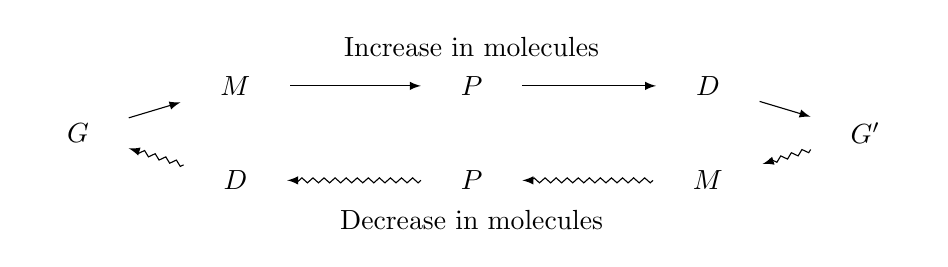
\begin{tikzpicture}

		\node at (0, 1.1) {Increase in molecules};

		\node[inner sep=.5cm] (AA) at (-3,.6) {$M$};
		\node[inner sep=.5cm] (BB) at (0,.6) {$P$};
		\node[inner sep=.5cm] (CC) at (3,.6) {$D$};
		\node[inner sep=.5cm] (DD) at (5,0) {$G'$};

		\node at (0, -1.1) {Decrease in molecules};

		\node[inner sep=.5cm] (EE) at (3,-.6) {$M$};
		\node[inner sep=.5cm] (FF) at (0,-.6) {$P$};
		\node[inner sep=.5cm] (GG) at (-3,-.6) {$D$};
		\node[inner sep=.5cm] (HH) at (-5,0) {$G$};

		\draw [arrows={-latex}] (HH) -- (AA);
		\draw [arrows={-latex}] (AA) -- (BB);
		\draw [arrows={-latex}] (BB) -- (CC);
		\draw [arrows={-latex}] (CC) -- (DD);
		\draw [arrows={-latex},decorate, decoration={zigzag, segment length=4, amplitude=.9,post=lineto, post length=2pt}] (DD) -- (EE);
		\draw [arrows={-latex},decorate, decoration={zigzag, segment length=4, amplitude=.9,post=lineto, post length=2pt}] (EE) -- (FF);
		\draw [arrows={-latex},decorate, decoration={zigzag, segment length=4, amplitude=.9,post=lineto, post length=2pt}] (FF) -- (GG);
		\draw [arrows={-latex},decorate, decoration={zigzag, segment length=4, amplitude=.9,post=lineto, post length=2pt}] (GG) -- (HH);
	\end{tikzpicture}
	\caption{Diagram of the effects of molecule populations in a gene regulatory network.}
	\label{fig:GRN_cycle}
\end{figure}

%As in Section~\ref{sec:chem_multiscale} we use the constrained multiscale approach to model the system.
Due to the small scale of the system and the speed of the reactions, we are only able to measure the total amount of protein, $T$, and mRNA, $M$, while the number of dimers and whether or not the gene is switched on must be considered to be missing data. For this scenario, the likelihood function is intractable and so we must use a multiscale approximation of the system. Here we choose the constrained multiscale approximation due to its success in the previous example.

The formulation here is slightly more complex. We define a fast subsystem which acts on the fast variables $\mathcal{F} = [P, D, G]$ and incorporates reactions $R_1$-$R_4$. For the true parameter values we have chosen, 90\% of reactions which occur in a particular time frame are one of these four reactions.
\[
	\text{Fast subsystem:} \quad P+P\xleftrightarrows[k_2]{k_1} D, \quad G+D\xleftrightarrows[k_4]{k_3} G'.
\]
We also define the slow variables, $T = P+2D+2(1-G)$ and $M$ which are held constant by these fast reactions.

When we observe a cell, we cannot distinguish between the fast species and so don't know which of the first four reactions are happening. Due to this, we observe how many of reactions $R_5$-$R_8$ occur for each combination of the two slow variables $\mathcal{S} = [T, M]$. Since we don't observe $P$ and $G$ for every reaction, the propensities must be altered to take this into account,
\begin{align}
	\hat{\alpha}_5 = k_5\mathbb{E}[G|T=t],\quad&\quad \alpha_6 = k_6M, \notag\\
	\hat{\alpha}_7 = k_7\mathbb{E}[P|T=t], \quad&\quad \alpha_8 = k_8M.\label{eqn:grn_propensities}
\end{align}

To calculate these expectations, we note that the fast subsystem is a deficiency zero system~\cite{anderson2010product}, and is also reversible. i.e. The system has four complexes, 
\[
	C_1 = P+P, \quad C_2 = D, \quad C_3 = G+D \quad \text{and} \quad  C_4 = G',
\]
there are two linkage classes (or two sets of reversible reactions), and the space spanned by the stoichiometries is two dimensional,
\[
	\text{span}\left\{\pm[-2, 1, 0, 0]^\top, \pm[0, -1, 0, -1]^\top\right\},
\]
hence the deficiency is $d = 4 - 2 - 2 = 0$. This means that, by \cite{anderson2010product}, the conditional probabilities have the closed form equation,
\[
	\mathbb{P}[\mathcal{F}|T=t] \propto \text{Poisson}(P_t;\bar{p})\text{Poisson}(D_t;\bar{d})\text{Poisson}(G_t;\bar{g})\text{Poisson}(1-G_t;1-\bar{g}),
\]
from which we can calculate the expected values of $P_t$, $D_t$, and $G_t$. The fast variables $P_t$, $D_t$ and $G_t$ are constrained to the line defined by $T=P+2D+2(1-G)=t$. The concentrations $\bar{p}$, $\bar{d}$ and $\bar{g}$, must be calculated as the solution to the nonlinear system produced by examining the steady state behaviour of the fast subsystem,
\begin{align}
	T &= p + 2d + 2(1-g), \notag\\
	\frac{\text{d}p}{\text{d}t} &= -2k_1p^2+2k_2d = 0, \notag\\
	\frac{\text{d}d}{\text{d}t} &= k_1p^2 - k_2d - k_3gd + k_4(1-g) = 0, \notag\\
	\frac{\text{d}g}{\text{d}t} &= -k_3gd + k_4(1-g) = 0, \label{eqn:grn_nonlinear_system}
\end{align}
subject to $p \in [0, T]$, $g \in [0, 1]$, and $0 \leq d \leq \text{floor}(T/2)$.

With these effective propensities, given in Equation~\eqref{eqn:grn_propensities}, we can calculate the posterior distribution as given in Equation~\eqref{eqn:chem_posterior}, again assigning Gamma priors to the eight reaction rates. We note that the reaction rates for the fast variables do not appear in the posterior density explicitly which only uses the propensities $\alpha_5$-$\alpha_8$, however they appear through the solution to the nonlinear system in Equation~\eqref{eqn:grn_nonlinear_system}.

\subsubsection{Target Distribution}

As in the previous chemical system example we use the target distribution as defined in Equation~\eqref{eqn:chem_posterior}. The application here is slightly more involved as discussed previously in Section~\ref{sec:grn}. We have an eight dimensional parameter space, with one reaction rate corresponding to one of eight reactions. The first four reactions, $R_1$-$R_4$, are combined into a fast subsystem for which we do not observe the time or identifier for which reaction has fired. We instead use the constrained multiscale approach to approximate what has happened in this subsystem between occurrences of the slow reactions firing (reactions $R_5$-$R_8$). For this reason, we apply the form in Equation~\eqref{eqn:chem_posterior} to reactions $R_5$-$R_8$, and allow the rates for reactions $R_1$-$R_4$ to implicitly influence the posterior density through the effective propensities, $\hat{\alpha}_5$ and $\hat{\alpha}_7$.

As we mentioned earlier, for this problem we only consider the CMA's approximation to the system dynamics.

The priors for this problem were chosen to be fairly uninformative with respect to the likelihood function for each reaction rate. A list of the hyper-parameters corresponding to each Gamma prior can be found in Table~\ref{tab:grn_priors}.

\begin{table}[!h]
\centering
\begin{tabular}{|l|R{1.8em}|R{1.8em}|R{1.8em}|R{1.8em}|R{1.8em}|R{1.8em}|R{1.8em}|R{1.8em}|}
	\hline
	Dimension $i$ & 1 & 2& 3& 4 & 5 & 6 & 7 & 8 \\ \hline
	$\alpha_i$ & 2 & 100 & 100 & 3 & 3 & 3 & 2 & 2\\ \hline
	$\beta_i$ &50 & 0.02 & 1 & 1 & 0.6 & 1 & 50 & 50 \\ \hline
\end{tabular}
\caption{Hyper parameters for the Gamma priors on each of the reaction rates in the GRN example in Section~\ref{sec:grn}.}
\label{tab:grn_priors}
\end{table}

\begin{figure}[htb]
\centering
\makebox[\textwidth][c]{\includegraphics[width=1.2\textwidth]{"images/GRN_posterior"}}%
\caption{Marginal densities of the posterior distribution for the GRN example in Section~\ref{sec:grn}.}
\label{fig:GRN_posterior}
\end{figure}

The one- and two-dimensional marginal distributions for the full posterior distribution are displayed in Figure~\ref{fig:GRN_posterior}. The posterior does not contain many interesting correlation structures, however several dimensions have leptokurtic tails which are difficult for the standard PAIS algorithm to sample from. The marginal densities also vary over very different scales, which might require us to use a variant of the LPAIS algorithm.

\subsubsection{Implementation}

%% proposal methods
%For the posterior distribution in \eqref{eqn:chem_QEA_posterior}, we consider several proposal methods. First we implement both the PAIS and MH algorithms with a Gaussian proposal distribution. In the case of the PAIS algorithm, this is a Gaussian mixture proposal distribution. The proposal distribution uses a covariance matrix which has been constructed using the sample covariance of a sample produced using a standard RWMH algorithm. We also compare the PAIS and MH algorithms when using a transport map proposal distribution. This proposal method was discussed in detail in Chapter~\ref{sec:TransportPAIS}.
%
%
%Figure~\ref{fig:chem_coupling} shows how we define a bijective map, $T'$, between parameter space $\mathcal{X}$ and a reference space $R$. In practice we cannot ensure that the approximate map $\tilde{T}'$ is uniquely invertible over the whole of $R$ and so $\tilde{T}'$ is not truly bijective. This leads to problems for our strictly positive state space, $\mathcal{X} \subset \mathbb{R}_+^d$, since proposals in $R$ do not necessarily map back on to $\mathcal{X}$. This motivates the use of a third intermediate space. When using the transport map proposal distribution, we prefix the proposal method with a T, e.g. MH-RW (RWMH) and MH-TRW, as well as PAIS-RW and PAIS-TRW.
%
%We also consider how these algorithms perform when they are applied to the log of the reaction rates. We choose to use this log transformation since it converts our strictly positive parameter space, $\mathcal{X}$, into an intermediate space $\mathcal{Y} \subset \mathbb{R}^d$. This allows us to define $T$ between two subsets of $\mathbb{R}^d$, which means that even if $\tilde{T}$ is not uniquely invertible in some region of $R$, all possibilities are valid proposals. As before, the proposal distributions are labelled with a T for transport map and when using the intermediate space we prepend `log' to the proposal method, e.g. MH-logRW and MH-logTRW, with, PAIS-logRW and PAIS-logTRW.
We apply the eight RW and logRW proposal distributions, with and without transport map acceleration, which were discussed in Section~\ref{sec:chem_multiscale} to this posterior. Again the intermediate log space is required so that our transport map is a function $T\colon\mathbb{R}^d\rightarrow\mathbb{R}^d$, rather than a map from $\mathbb{R}_+^d$ to $\mathbb{R}^d$.

%% choices made in transport map
%For this problem, we continue to use monomials in each dimension in our transport map construction. We use polynomials of total order $p=4$ as the basis functions, i.e.
%\[
%	T_i(\theta) = \sum_{\mathbf{j}\in\mathcal{J}^{\text{TO}}_i(p)} \gamma_{i,\mathbf{j}}\psi_{\mathbf{j}}(\theta) \quad \text{where} \quad \psi_\mathbf{j}(\theta) = \prod\limits_{k=1}^i \theta_k^{j_k},
%\]
%and
%\[
%	\mathcal{J}^{\text{TO}}_i(p) = \{\mathbf{j} \in \mathbb{N}^d_0\ |\ \|\mathbf{j}\|_1 \leq p, \ \text{and}\ j_k = 0\ \forall k > i\}.
%\]
%Since $\mathcal{X}$ is four-dimensional, this yeilds a total of 125 map coefficients across the four index sets. This number can be reduced by using smaller index sets as discussed in~\cite{parno2014transport}.
The transport map setup has not changed from the previous example. However, due to the scaling of the weight we have had to be more careful about which samples we use to build our map. We require that the objective function $C(T)$, from Equation~\eqref{eqn:TPAIS_objective} is convex, which requires that the second derivative, given in Equation~\eqref{eqn:TPAIS_hessian}, is positive definite. This positive definite property depends on all weights in our sample being strictly positive, which is not always possible on a computer. For this reason we filter out any samples from the optimisation problem where the weight is a numeric zero. This does not affect the validity of the map since a weight zero would not contribute to the expectation, and we do not require (and could not enforce) an exact map.

In all eight algorithms we adapt the proposal variances during the burn-in phase of the algorithms to avoid behaviour like that seen in Example~\ref{sec:ex_W1} where we needed a huge ensemble size to approximate the posterior with our mixture of isotropic Gaussian kernels.

%% choice of resampler?
%As with the mixture model in Section~\ref{sec:app_mixture}, we will use the AMR resampler with an ensemble size of $M=500$. This increase in ensemble size from Chapter~\ref{sec:PAIS} compensates for the increase in parameter dimension.
We again use the AMR resampler, this time with an ensemble size of $M=2500$. The increase in ensemble size again compensates for the increase in dimension (from four to eight parameters.)

%% analysis method
%To measure the convergence of the sampling methods in this section, we will compare the convergence of the mean of each parameter. We approximate $\mathbb{E}(\mathbf{k})$ using 2.4 billion samples from the MH-RW algorithm.
As in the previous chemical reaction example, we measure convergence of the algorithms only through the convergence of the mean, for computational ease. We use the sample Mahalanobis distance, with `true' covariance and `true' mean built from a sample of size 2.4 billion using the MH-RW algorithm.

\subsubsection{Convergence results}

The scaling parameter selection is done by optimising the acceptance rate for the MH algorithms, and optimising the effective sample size for the PAIS algorithms. The optimal parameters are given in Table~\ref{tab:grn_scaling_parameters}.

\begin{table}[!h]
	\centering
	\begin{tabular}{lrrrrrrrr}
	\toprule
		 & \multicolumn{4}{c}{MH} & \multicolumn{4}{c}{PAIS} \\ \cmidrule(lr){2-5} \cmidrule(lr){6-9}
		& RW & logRW & TRW & log-TRW & RW & logRW & TRW & log-TRW \\ \midrule
		$\beta_{\%}^*$	 	& 1.0e-1 & 3.9e-1 & 1.0e-0 &6.0e-1 & - & - & - & - \\
		$\beta_{\text{ESS}}^*$	& - 	        & -           & -            & -            & 1.0e-0 & 1.3e-0 & 8.0e-1 & 5.0e-1 \\
		ESS/$M$		 		& - 	        & -           & -            & -            & 3.5e-4 & 4.7e-2 & 4.8e-2 & 1.6e-1  \\
	\bottomrule
	\end{tabular}
	\caption{Scaling parameters for the sampling algorithms applied to the GRN example in Section~\ref{sec:grn}.}
	\label{tab:grn_scaling_parameters}
\end{table}

From the effective sample sizes shown in Table~\ref{tab:grn_scaling_parameters} we can see the improvement to the efficiency of the algorithm both by proposing on the log space, and by transforming the parameter space into something closer to Gaussian.

Due to the numerical cost of calculating the full relative $L^2$ errors for this posterior, we quantify the convergence speeds of these algorithms using the sample Mahalanobis distance between the sample mean and the `true' mean. This convergence analysis is shown in Figure~\ref{fig:grn_L2}.

\begin{figure}[!htb]
\centering
\subfigure[Sampling algorithms on $\mathcal{X}$.]{\includegraphics[width=0.495\textwidth]{"images/GRN_convergence"}}
\subfigure[Sampling algorithms on $\mathcal{Y}$.]{\includegraphics[width=0.495\textwidth]{"images/GRN_convergence_log"}}
\caption{Convergence of the GRN example described in Section~\ref{sec:grn}.}
\label{fig:grn_L2}
\end{figure}

The first thing to note is that the first PAIS measurement happens after 2500 samples, whereas the first MH measurement occurs after 50 samples. This is due to the much larger ensemble size required to sample in higher dimensions. We believe that an ensemble size of 2500 is over-cautious in this example and we could have used a smaller ensemble size. We also think that the required ensemble size to sample from these posteriors is reduced by the use of the transport map. This is due to the way the tail behaviour is improved by the transformation.

The second obvious feature of these convergence plots is that the PAIS algorithms outperform the MH algorithms by a large margin - roughly a reduction of two orders of magnitude in the relative error over the same number of samples. A less positive result is that for this example the PAIS-TRW algorithm has found a map which has prevented further convergence of the mean. This is likely because one dimension of the transport map is sending proposals onto the negative real line and so all samples are being assigned a zero weight. This is behaviour which was anticipated, and it is always suggested that the transport map is constructed as a map $T\colon\mathbb{R}^d\rightarrow\mathbb{R}^d$ rather than $T\colon\mathcal{X}\rightarrow\mathbb{R}^d$ where $\mathcal{X}\subset\mathbb{R}^d$. The large increase in the effective sample size observed between the PAIS-logRW and PAIS-logTRW algorithms is converted into an estimate which is twice as accurate after 1 million samples.

A similar pattern is seen in the MH algorithms, where the MH-TRW performs the worst, and the MH-logTRW algorithm performs the best, although only marginally.

\section{Conclusions}

In this chapter we have demonstrated the process of applying the PAIS algorithm to realistic modelling situations. We saw how the standard PAIS algorithm can perform well for multimodal distributions in Section~\ref{sec:app_mixture}, in this case we only needed a RW proposal distribution, but it is possible to use the LPAIS algorithm or transport map based proposals if the tails of the posterior are not well behaved.

We have also seen how the transport map converts posteriors which are badly scaled, have complicated correlation structures and possibly have non-Gaussian tails, into posteriors which we can sample effectively. This was demonstrated for two chemical reaction networks in Sections~\ref{sec:chem_multiscale} and \ref{sec:grn}

These algorithms, when compared with the standard MC toolbox, have consistently performed the best, in the last GRN example realising estimates with more than two orders of magnitude better accuracy.

\bibliographystyle{siam}
\bibliography{refs}
\end{document}
